% Modelo adaptado pelo prof. Dr. Alysson Filgueira Milanez
% Campus Pau dos Ferros

\documentclass[        
    a4paper,          % Tamanho da folha A4
    12pt,             % Tamanho da fonte 12pt
    chapter=TITLE,    % Todos os capitulos devem ter caixa alta
    section=Title,    % Todas as secoes devem ter caixa alta somente na primeira letra
    subsection=Title, % Todas as subsecoes devem ter caixa alta somente na primeira letra
    oneside,          % Usada para impressao em apenas uma face do papel
    english,          % Hifenizacoes em ingles
    brazilian,        % Ultimo idioma eh o idioma padrao do documento
    fleqn,            % Comente esta linha se quiser centralizar as equacoes. Comente também a linha 65 abaixo
    hyphens,
    sumario=tradicional,
]{abntex2}

\input{lib/preambulo}

\setlength{\mathindent}{0pt} %Complementa o alinhamento de equações para totalmente a esquerda.

\trabalhoacademico{tccgraduacao}

\removerbordasdohyperlink{sim} 

\cordohyperlink{nao}

\ies{Universidade Federal Rural do Semi-Árido}
\iessigla{UFERSA}
\centro{Pró-Reitoria de Graduação}
\departamento{Departamento de Computação}

\graduacaoem{Ciência da Computação}
\habilitacao{bacharel} 

\autor{Paulo Henrique Almeida de Andrade} 
\titulo{IMPLEMENTAÇÃO DE UM SISTEMA DISTRIBUÍDO PARA INTEGRAÇÃO DE INSTRUMENTAÇÕES EMBARCADAS EM VOO DE VANTs}
\subtitulo{}
\data{2026}
\local{Mossoró}

% Exemplo: \dataaprovacao{08 / 10 / 2025}
\dataaprovacao{\underline{  }}

\orientador{Xxxxxxx Xxxxxx Xxxxxxx}
\titulacaoOrientador{Prof. xx.}
\orientadories{UFERSA}
\orientadorcentro{)} % opcional
\orientadorfeminino{nao} % Coloque 'sim' se for do sexo feminino

%\coorientador{}
%\titulacaoCoOrientador{Prof. xx.}
%\coorientadories{SIGLA}
%\coorientadorcentro{Centro do Coorientador (SIGLA)} % opcional
%\coorientadorfeminino{nao} % Coloque 'sim' se for do sexo feminino


% Exemplo de uso:
% \membrodabancadois{Fulano de Tal}
% \titulacaoBancaDois{Prof. xx.}
% \membrodabancadoiscentro{CMPF}
% \membrodabancadoisies{Universidade Federal Rural do Semi-Árido - UFERSA}

\membrodabancadois{Xxxxxxx Xxxxxx Xxxxxxx}
\titulacaoBancaDois{Prof. xx.}
\membrodabancadoiscentro{}
\membrodabancadoisies{SIGLA}
\membrodabancatres{Xxxxxxx Xxxxxx Xxxxxxx}
\titulacaoBancaTres{Prof. xx.}
\membrodabancatrescentro{}
\membrodabancatresies{SIGLA}
\membrodabancaquatro{}
\membrodabancaquatrocentro{}
\membrodabancaquatroies{SIGLA}
\membrodabancacinco{Prof. Dr. Xxxxxxx Xxxxxx Xxxxxxx}
\membrodabancacincocentro{Teste}
\membrodabancacincoies{Universidade do Membro da Banca Cinco (SIGLA)}
\membrodabancaseis{Prof. Dr. Xxxxxxx Xxxxxx Xxxxxxx}
\membrodabancaseiscentro{}
\membrodabancaseisies{Universidade do Membro da Banca Seis (SIGLA)}

% Para espacaomento duplo nas referencias
% \let\OLDthebibliography\thebibliography
% \renewcommand\thebibliography[1]{
% \OLDthebibliography{#1}
% \setlength{\itemsep}{24pt} % Space between items
% \setlength{\parskip}{0pt} % Space between paragraphs
% }


\begin{document}	

	% Elementos pré-textuais
	\imprimircapa
	\imprimirfolhaderosto{}
	%\imprimirfichacatalografica{1-pre-textuais/ficha-catalografica} %  gerada pela biblioteca 
	\imprimirfolhadeaprovacao 
	\imprimirdedicatoria{1-pre-textuais/dedicatoria}
	\imprimiragradecimentos{1-pre-textuais/agradecimentos}
	\imprimirepigrafe{1-pre-textuais/epigrafe}
	\imprimirresumo{1-pre-textuais/resumo}
	\imprimirabstract{1-pre-textuais/abstract}
	\renewcommand*\listfigurename{Lista de Figuras} %Se você comentar esta linha o título da lista fica: LISTA DE ILUSTRAÇÕES
	\imprimirlistadeilustracoes
	\imprimirlistadetabelas
	\imprimirlistadequadros
	%\imprimirlistadealgoritmos
	%\imprimirlistadecodigosfonte
	\imprimirlistadeabreviaturasesiglas
	% \imprimirlistadesimbolos{1-pre-textuais/lista-de-simbolos}   
	\imprimirsumario
	
	\setcounter{table}{0}% Deixe este comando antes da primeira tabela.
	
	%Elementos textuais
	\textual
	\chapter{Introdução}
\label{cap:introducao}

\section{Contextualização}
Explicação do contexto: aerodesign, voos de UAV, telemetria

\subsection{Problematização}
Hipótese da solução

\subsubsection{Metodologia}
Requisitos (SMART)


	\chapter{Embasamento Teórico}
\label{cap:embasamento-teorico}
O desenvolvimento de um sistema de telemetria distribuído para ensaios em voo de Veículos Aéreos Não Tripulados (VANTs) pressupõe o domínio de conceitos estruturais de sistemas computacionais e telecomunicações. A instrumentação embarcada atua sob limitações físicas e energéticas inerentes à operação aeronáutica, fatores que condicionam diretamente as decisões de projeto de hardware e software. Desta forma, o embasamento teórico fornece a fundamentação técnica necessária para balizar e justificar as escolhas de padrões arquiteturais, protocolos de comunicação, gerenciamento de processamento em tempo real e técnicas de otimização de dados aplicadas na concepção da solução.

\section{Restrições em Sistemas Embarcados Aeronáuticos}
A instrumentação de Veículos Aéreos Não Tripulados (VANTs) é limitada pelas características físicas e operacionais da aeronave. Ao contrário de plataformas terrestres estáticas, o projeto de hardware aeronáutico é regido pelo critério SWaP (Size, Weight, and Power), que atua como o principal fator de decisão para a viabilidade e integração de sistemas eletrônicos embarcados \cite{raymer_aircraft_design}.

A dimensão e a massa dos componentes afetam o centro de gravidade, a estabilidade e a capacidade de carga útil da plataforma. Essa restrição exige a minimização da área ocupada pela placa de circuito impresso (PCB) e a seleção de componentes com alto nível de integração. Do ponto de vista energético, a fonte de alimentação do sistema de aquisição frequentemente compartilha as baterias do sistema de controle da aeronave. O acionamento de atuadores mecânicos, somado ao uso de microcontroladores de duplo núcleo e módulos de radiofrequência de longo alcance, gera picos de corrente e ruído conduzido no barramento. Para manter a estabilidade térmica e elétrica sob essas condições limitantes, o projeto de distribuição de potência requer topologias de alimentação isoladas, como a arquitetura Dual-Rail, que separa a alimentação sensível dos sensores das cargas com alta demanda transiente \cite{uav_swap_telemetry}.

\section{Arquitetura de Software e Sistemas Distribuídos}

A integração de sistemas heterogêneos, que operam desde a coleta de dados embarcada até a visualização analítica na estação em solo, exige a adoção de padrões arquiteturais rigorosos. A estruturação lógica do \textit{software} deve garantir o baixo acoplamento entre componentes isolados, assegurando consistência na troca de informações e escalabilidade para a adição de novas fontes de dados.

\section{Sistemas Distribuídos e \textit{Middleware}}

Em cenários onde múltiplos nós autônomos produzem e consomem dados de forma assíncrona, a coordenação das ações ocorre fundamentalmente pela troca de mensagens sobre uma rede de comunicação \cite{coulouris_distributed}. Devido à heterogeneidade dos protocolos físicos e estruturas de pacotes gerados pelos módulos produtores, introduz-se a camada de \textit{middleware}. Este componente atua como um integrador intermediário projetado para abstrair as especificidades de \textit{hardware} e as conexões de baixo nível. Sua função restringe-se a capturar, padronizar e rotear o tráfego de dados para a aplicação cliente, unificando o fluxo de informações no sistema \cite{coulouris_distributed}.

\subsection{Arquitetura Hexagonal (\textit{Ports and Adapters})}

No desenvolvimento tradicional de \textit{firmware}, é comum a ocorrência de acoplamento severo entre as regras lógicas de operação e os registradores específicos do \textit{hardware}. Para mitigar esse problema, aplica-se a Arquitetura Hexagonal, ou \textit{Ports and Adapters}, cujo princípio central é a inversão de dependência \cite{martin_clean_architecture}. O núcleo lógico da aplicação (domínio) é totalmente isolado de agentes externos. A comunicação com o microcontrolador, sensores e módulos de comunicação ocorre exclusivamente por meio de contratos formais (portas), que são implementados na periferia do sistema por bibliotecas específicas (adaptadores) \cite{martin_clean_architecture}. Além de garantir a modularidade, esta topologia viabiliza metodologias de teste como \textit{Hardware-in-the-loop} (HIL), permitindo a validação do domínio lógico mediante a injeção de adaptadores de \textit{software} emulados em substituição ao \textit{hardware} físico.

\subsection{Padrão \textit{Model-View-Controller} (MVC)}

Na estação de controle em solo, a recepção de fluxos contínuos de telemetria concorre diretamente com as demandas de renderização gráfica. Se as rotinas bloqueantes de entrada e saída (I/O) de rede forem executadas na mesma \textit{thread} de atualização da interface, o acúmulo de processamento induzirá latência e consequente descarte de pacotes no \textit{buffer} do sistema operacional. O padrão \textit{Model-View-Controller} (MVC) isola matematicamente essas responsabilidades \cite{fowler_eaa}. O \textit{Model} concentra a lógica de negócios, a aquisição via rede e o armazenamento em memória; a \textit{View} restringe-se à renderização passiva de matrizes geométricas na tela; e o \textit{Controller} atua como orquestrador de eventos assíncronos, transferindo cópias seguras de dados do modelo para a interface em uma taxa de atualização controlada \cite{fowler_eaa}.

\section{Telecomunicações e Protocolos de Rede}

A comunicação de dados entre uma aeronave em movimento e uma estação terrestre exige o contorno de atenuações de sinal e ruídos presentes no canal de rádio. A escolha das tecnologias da camada física e de transporte determina a resiliência e a latência do tráfego de telemetria no sistema distribuído.

\subsection{Modulação LoRa e o Teorema de Shannon-Hartley}

O Teorema de Shannon-Hartley estabelece a capacidade máxima teórica de transmissão de um canal em função da sua largura de banda e da relação sinal-ruído (SNR) disponível. Em ensaios em voo, o afastamento radial da aeronave em relação à estação base degrada rapidamente a potência do sinal recebido, reduzindo drasticamente a SNR. Para manter a integridade da comunicação sob estas condições, aplica-se a técnica de espalhamento espectral (\textit{Spread Spectrum}), que compensa a deficiência de potência ampliando a largura de banda ocupada pela transmissão \cite{haykin_communication}.

A modulação LoRa, operante em bandas Sub-GHz (como a faixa não licenciada de 915 MHz), utiliza este princípio físico. A escolha por frequências mais baixas prioriza a capacidade de penetração de sinal e o alcance em linha de visada (BVLOS), sacrificando em contrapartida a taxa máxima de transferência de dados (\textit{bit rate}) quando comparada a protocolos de 2,4 GHz, como Wi-Fi ou módulos convencionais de curto alcance \cite{lora_uav_performance}.

\subsection{O Protocolo MAVLink}

Na camada lógica de rede, a estruturação dos dados afeta diretamente o consumo da banda de radiofrequência. Protocolos genéricos de Internet das Coisas (IoT), como o MQTT, operam sobre conexões TCP e frequentemente utilizam serialização baseada em texto (como JSON), gerando um \textit{overhead} insustentável para enlaces Sub-GHz. Em paralelo, protocolos como o LoRaWAN impõem topologias de rede complexas e limitações de ciclo de trabalho (\textit{duty cycle}) que introduzem alta latência.

Para telemetria contínua, o protocolo MAVLink fornece um mecanismo de empacotamento estritamente binário, leve e com comportamento de roteamento análogo ao UDP (\textit{User Datagram Protocol}), permitindo o envio rápido de mensagens sem a necessidade de estabelecimento prévio de conexão (\textit{handshake}) \cite{mavlink_dev_guide}. O protocolo opera em um modelo de publicação e assinatura nativo, baseando-se em identificadores de sistema (\textit{System ID}) e componente (\textit{Component ID}) para rotear os pacotes. Em sua estrutura, garante a verificação de integridade através de \textit{checksums} de redundância em seu cabeçalho, com a versão mais recente (v2) suportando a alocação de assinaturas de validação sem comprometer significativamente o tamanho do pacote \cite{mavlink_dev_guide}.

\section{Sistemas Embarcados e Tempo Real}

O gerenciamento de dados de sensores e o controle de dispositivos de comunicação requerem uma arquitetura de \textit{firmware} capaz de atender a múltiplos eventos de forma determinística, sem perda de amostras ou latências excessivas na resposta de \textit{hardware}.

\subsection{Microcontroladores e Barramentos de Comunicação}

A seleção da unidade de processamento baseia-se na capacidade de gerenciar periféricos síncronos e assíncronos sob condições de alta carga de dados. O emprego de microcontroladores modernos, como as arquiteturas \textit{dual-core} (ex: ESP32) ou baseadas em núcleos ARM Cortex-M (ex: STM32), permite o isolamento de tarefas computacionalmente distintas, alocando o processamento de baixo nível e a leitura de sensores em barramentos I2C ou SPI em núcleos dedicados, enquanto o gerenciamento da lógica de estado é executado paralelamente \cite{white_embedded_systems}. O barramento I2C, embora permita a redução da complexidade de \textit{hardware} ao compartilhar pinos entre múltiplos sensores, exige mecanismos robustos de tratamento de exceções no \textit{firmware} para evitar travamentos decorrentes de falhas de sincronismo ou ruído no silício \cite{st_stm32_bus_manual}.

\subsection{Sistemas Operacionais de Tempo Real (RTOS)}

A complexidade da orquestração de tarefas assíncronas — como o monitoramento da telemetria, a leitura de IMUs e a resposta a comandos do piloto — inviabiliza a abordagem \textit{bare-metal} tradicional em sistemas de maior porte. A adoção de um Sistema Operacional de Tempo Real (RTOS) permite a abstração do escalonamento, priorizando o atendimento a interrupções críticas de \textit{hardware} (como o término de uma transmissão de rádio) mediante o uso de primitivas de sincronização, tais como semáforos e filas de mensagens (\textit{queues}) \cite{barry_freertos}. Esta camada operacional assegura que o \textit{firmware} mantenha uma resposta previsível e estável frente à concorrência por recursos, minimizando o risco de \textit{jitters} no processamento de dados analíticos \cite{barry_freertos}.

\section{Otimização de Transmissão de Dados}

A quantização consiste na conversão de variáveis de ponto flutuante (\textit{float}) em tipos inteiros de tamanho fixo, técnica fundamental para reduzir a carga útil dos pacotes transmitidos em redes de banda estreita. Ao promover o escalonamento matemático das grandezas — multiplicando-as por potências de base 10 — é possível preservar a precisão física necessária, como a casa decimal centimétrica em coordenadas geodésicas, enquanto se reduz drasticamente o \textit{overhead} de memória e o tempo de serialização na transmissão \cite{oppenheim_signal_processing}. Esta abordagem mitiga os gargalos de largura de banda e reduz o custo computacional exigido para o empacotamento MAVLink, garantindo que o sistema atenda aos requisitos de \textit{throughput} sem comprometer a integridade dos dados de voo \cite{iot_data_compression_strategies}.

A fundamentação apresentada neste capítulo delimita os parâmetros técnicos que orientam o projeto. A análise das restrições de hardware aeronáutico, aliada às escolhas de arquitetura de software modular e protocolos de comunicação otimizados, estabelece a base lógica necessária para a implementação do sistema proposto. 

  	\chapter{Trabalhos Relacionados}
\label{cap:trabalhos-relacionados}
O desenvolvimento de Sistemas de Aquisição de Dados (SAD) e telemetria embarcada para Veículos Aéreos Não Tripulados (VANTs) de pequeno porte, especialmente no cenário de validação de projetos aeroespaciais (como na competição SAE Brasil AeroDesign), é um tema recorrente na literatura acadêmica. A necessidade empírica de validar modelos teóricos de aerodinâmica, desempenho e cargas estruturais impulsiona a criação de soluções customizadas que atendam a rigorosas restrições de SWaP (Size, Weight, and Power).

Trabalhos como o de Barbosa \cite{barbosa2022} e Bueno \cite{bueno2015} ilustram a abordagem clássica de engenharias universitárias para este problema. Barbosa \cite{barbosa2022} desenvolveu um sistema de telemetria focado no monitoramento em tempo real de variáveis de voo para projetos de aeromodelismo, com foco em eletrônica capaz de prover suporte computacional para testes. Semelhantemente, Bueno \cite{bueno2015} investigou a arquitetura de software embarcado de tempo real para instrumentação aeroelástica, frequentemente empregando módulos de comunicação da família XBee/ZigBee (2.4 GHz). Embora eficazes para coleta primária, essas soluções comumente adotam topologias fechadas (ponto-a-ponto monolítico) e protocolos de empacotamento em texto plano ou matrizes de bytes proprietárias, limitando severamente a escalabilidade caso o projeto demande integração de estações meteorológicas externas ou múltiplos VANTs simultâneos.

No que tange à camada física e de enlace, a adoção da modulação LoRa (Long Range) tem ganhado destaque acadêmico na instrumentação de VANTs por sua resiliência e alcance superior operando em frequências sub-GHz (915 MHz). Contudo, a literatura aponta o limitante crítico do LoRa: a restrita capacidade de canal, descrita pelo Teorema de Shannon-Hartley. Projetos de baixo custo geralmente contornam essa limitação enviando strings genéricas. Já os frameworks padronizados na indústria, como o protocolo MAVLink (adotado pelo ArduPilot e PX4), são comumente aplicados sobre links de telemetria dedicados de maior banda ou delegados a pesadas controladoras de voo prontas (Pixhawk), conforme analisado em estudos recentes de tráfego de rede para drones \cite{belwafi2022}. A geração de mensagens MAVLink diretamente em microcontroladores de borda (edge computing) em redes distribuídas de baixa banda continua sendo um desafio tecnológico no meio acadêmico de baixo orçamento.

Neste contexto, o presente trabalho contextualiza-se na mesma demanda de instrumentação aeronáutica acessível, porém diverge e inova substancialmente frente às implementações acadêmicas vigentes em três pilares metodológicos:

- Arquitetura Distribuída e Middleware: Ao contrário de módulos isolados que conectam a aeronave de forma unilateral ao visualizador no solo, o presente projeto implementa um modelo distribuído através do Shoulder (middleware). Essa camada centraliza, valida e formata os pacotes provenientes de nós completamente independentes (sistema da aeronave, obstáculos e clima terrestre), atuando como um barramento unificador de eventos, distanciando-se das arquiteturas monolíticas triviais.

- Empacotamento MAVLink com Otimização por Quantização: Diferentemente das soluções universitárias que evitam headers padronizados para economizar processamento, este trabalho aplica o dialeto MAVLink (v1/v2) como contrato de rede base, preservando a interoperabilidade. A limitação física do LoRa é solucionada de forma analítica: o domínio executa a quantização matemática em ponta, convertendo variáveis nativas em ponto flutuante ($float32$) para formatos inteiros escalonados ($int16\_t$ e $int32\_t$). Esta mitigação drástica de payload raramente é abordada em soluções equivalentes baseadas na abstração excessiva do ecossistema Arduino.

- Rigor de Engenharia de Software Orientado a Domínio: Na literatura de instrumentação maker, os firmwares são majoritariamente codificados em formato bare-metal procedural (Super Loops). Este trabalho opta pela implementação sob o FreeRTOS através de Arquitetura Hexagonal (Ports and Adapters). Essa separação técnica desvincula a regra de negócios aeroespacial dos periféricos elétricos, viabilizando ensaios de injeção de erros (Hardware-in-the-loop - HIL) antes da manufatura final da PCB, elevando o grau de determinismo e modularidade do sistema.

Portanto, o sistema abordado supera o escopo tradicional de data loggers isolados, assumindo a estrutura de um ecossistema de IoT aeronáutico altamente determinístico e focado no balanço ótimo entre restrição física, conformidade de rede aeroespacial e escalabilidade de engenharia de ensaios em voo.

	\chapter{Arquitetura distribuída}
\label{chap:arquitetura-distribuida}



\section{Projeto conceitual}
\begin{figure}[ht]
    \centering
    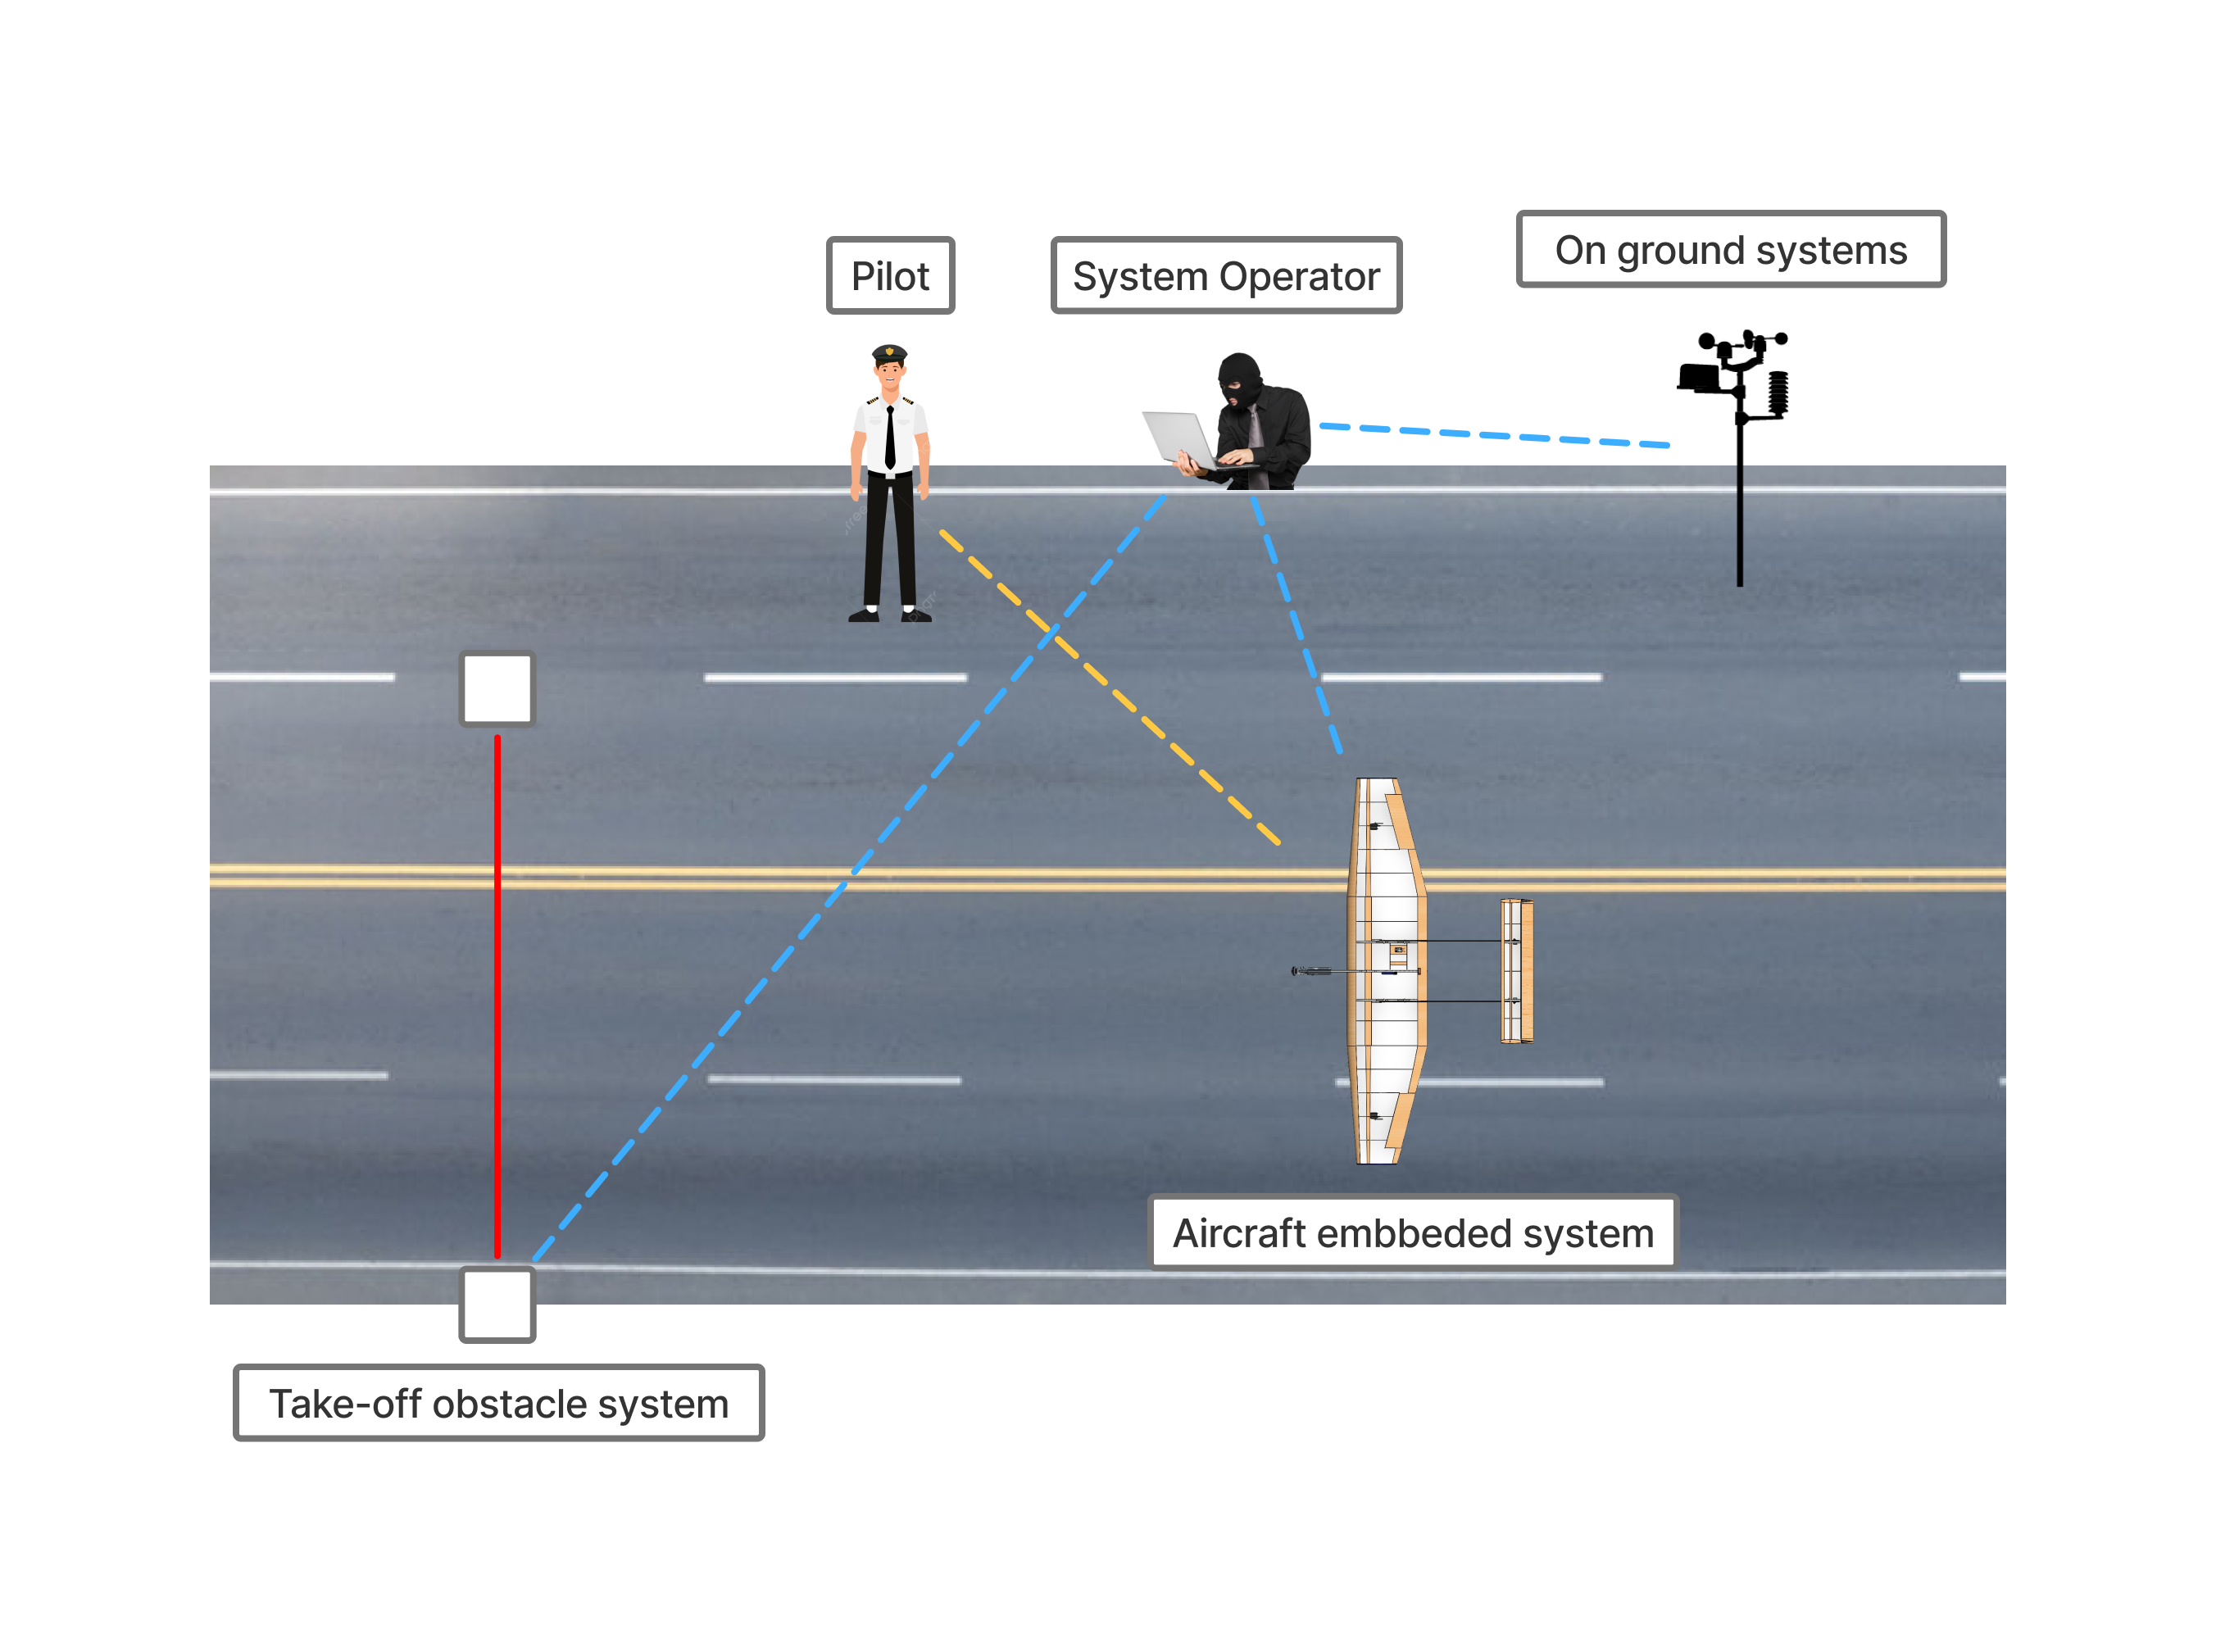
\includegraphics[width=0.9\textwidth]{images/design_conceitual.png}
    \caption{\textit{Design} conceitual da solução}
    \label{fig:design-conceitual}
\end{figure}

\section{Arquitetura de comunicação}
(Diagrama que se completa ao longo das subsections)

\subsection{Componentes distribuídos}
Ponta, middleware e client

\begin{figure}[ht]
    \centering
    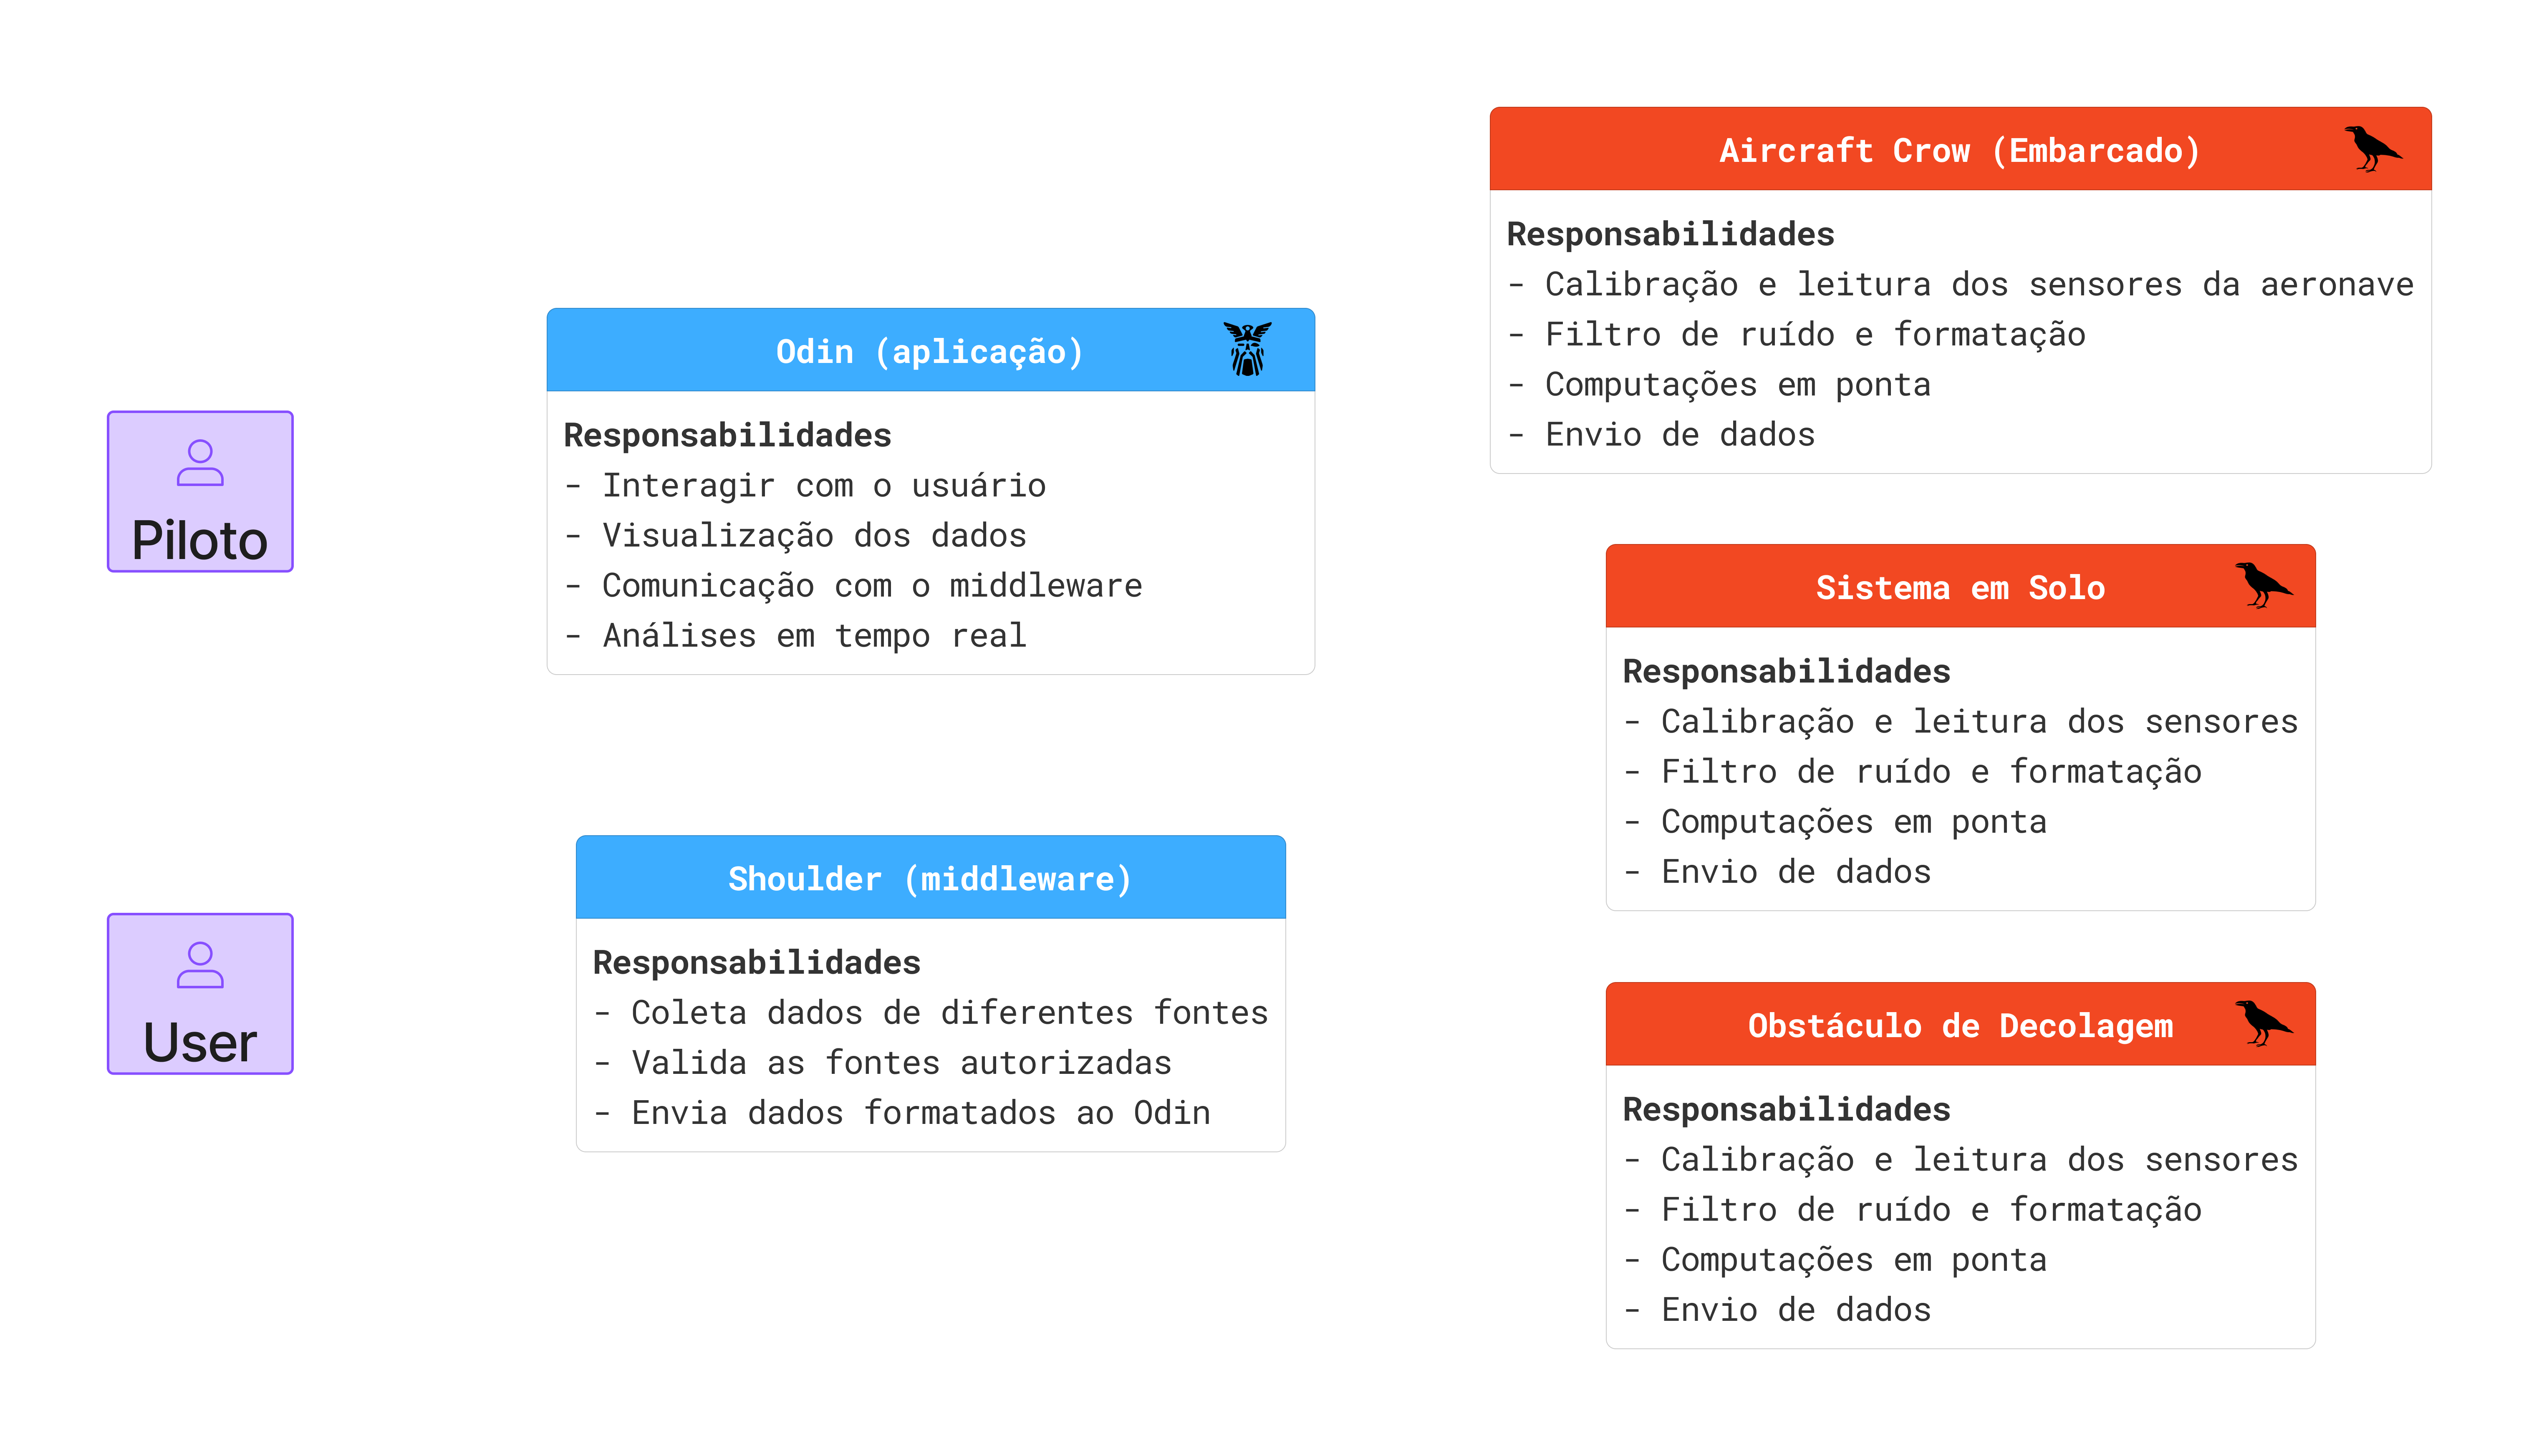
\includegraphics[width=0.85\textwidth]{images/componentes_design_comunicacao.png}
    \caption{Componentes distribuidos}
    \label{fig:componentes-distribuidos}
\end{figure}

\subsection{Camada física}
Escolha da antena e módulo RF

\begin{figure}[ht]
    \centering
    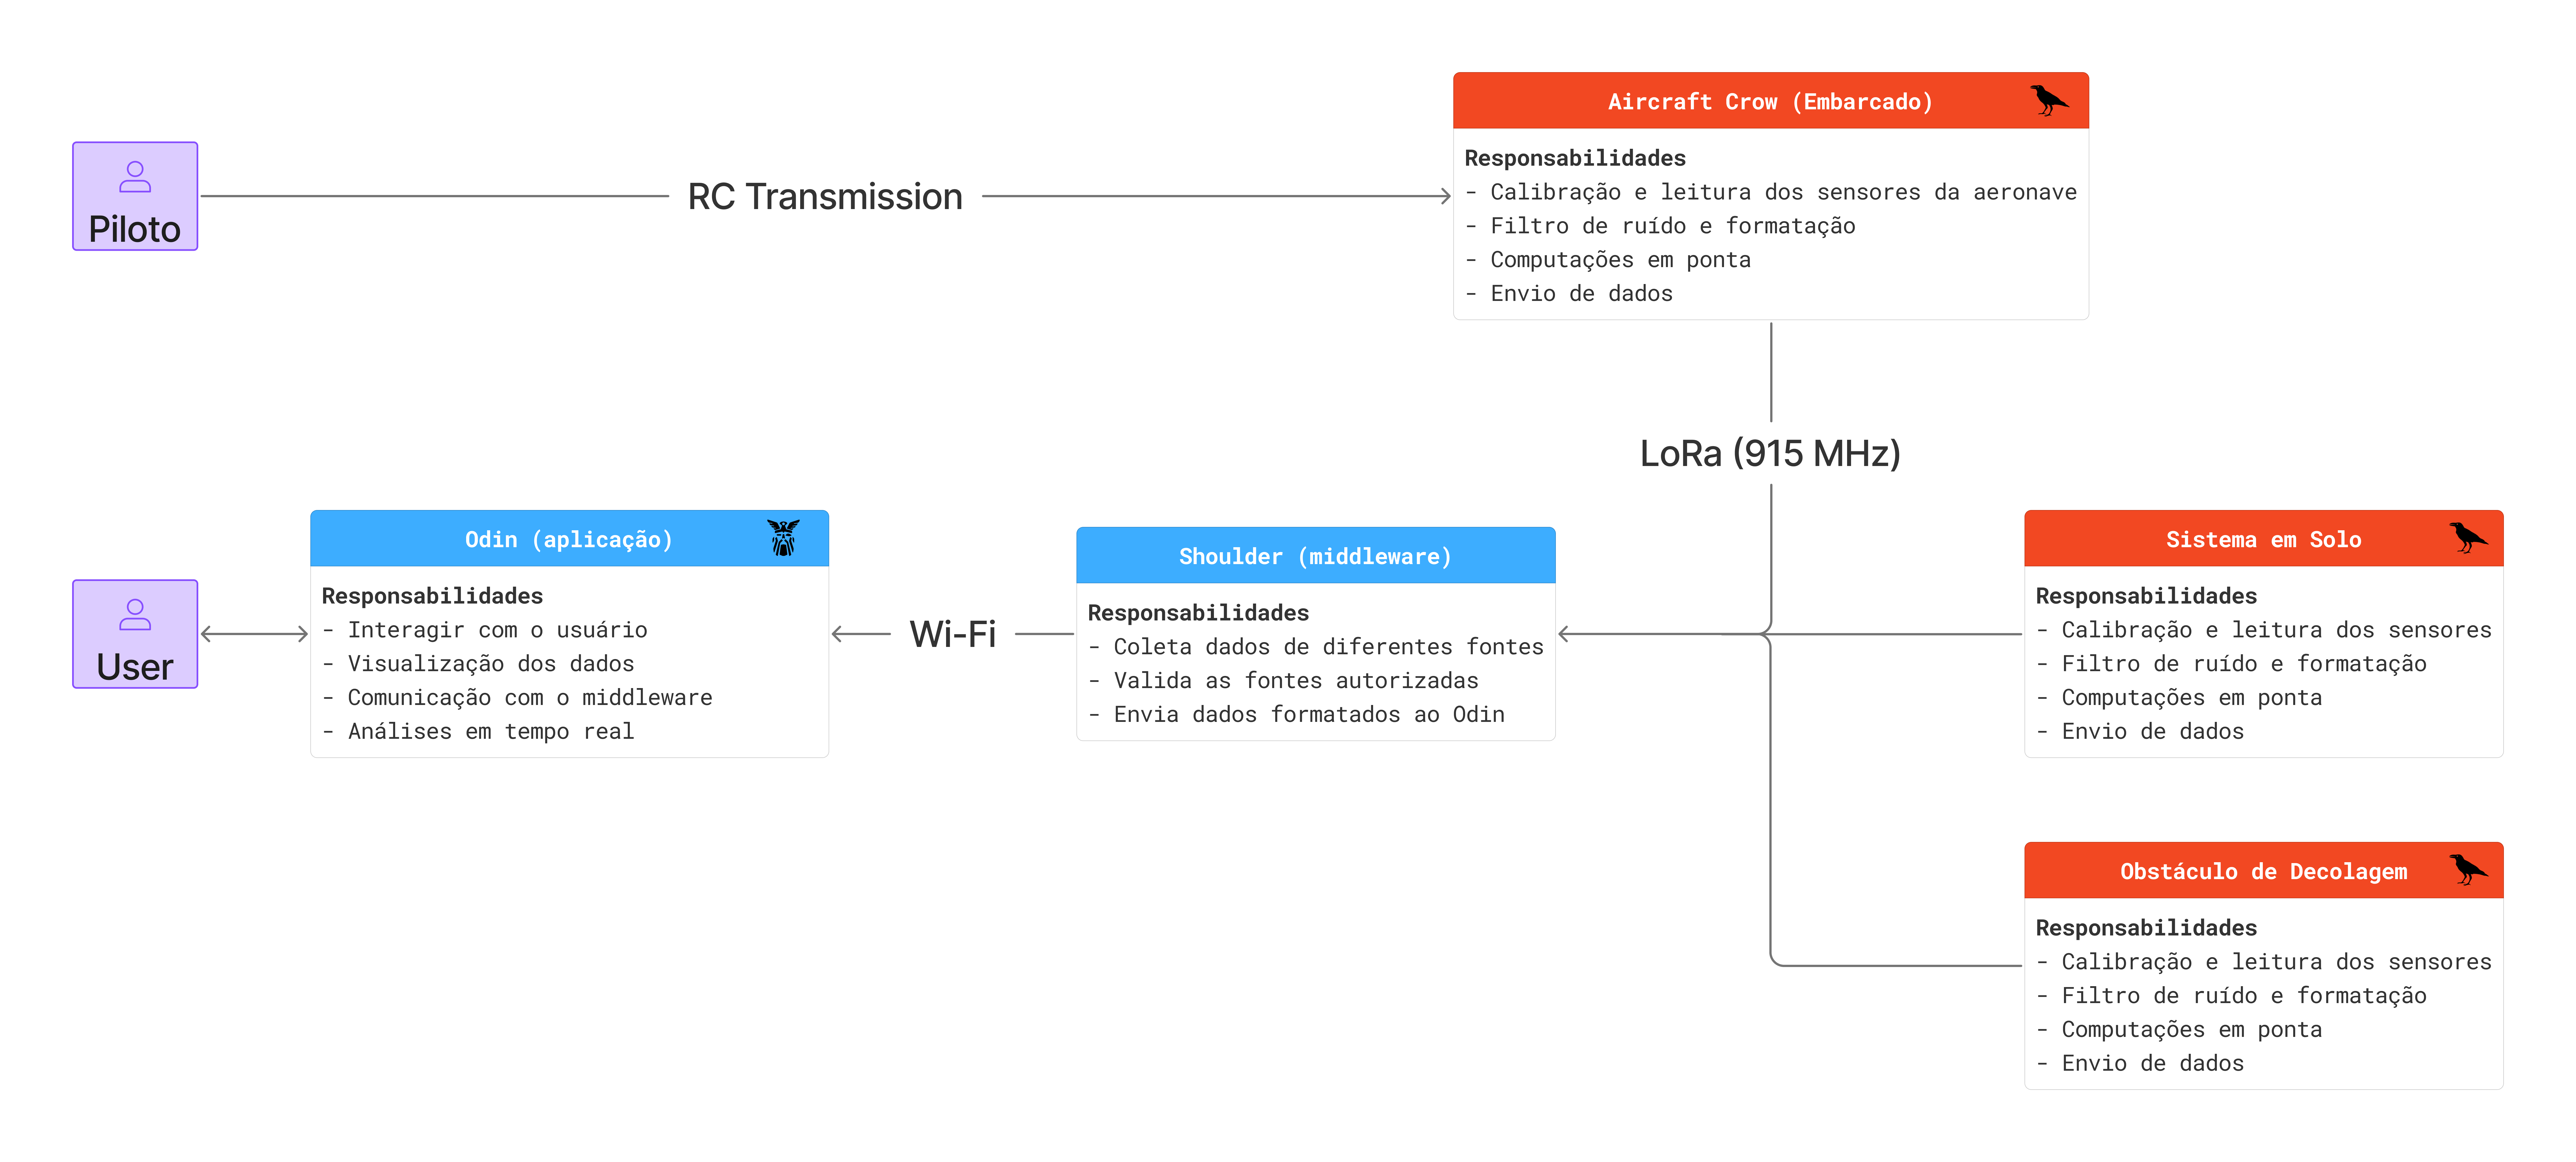
\includegraphics[width=0.85\textwidth]{images/camada_fisica_design_comunicacao.png}
    \caption{Camada física do sistema}
    \label{fig:camada-fisica}
\end{figure}

\subsection{Camada de transporte}
Escolha dos protocolos

\begin{figure}[ht]
    \centering
    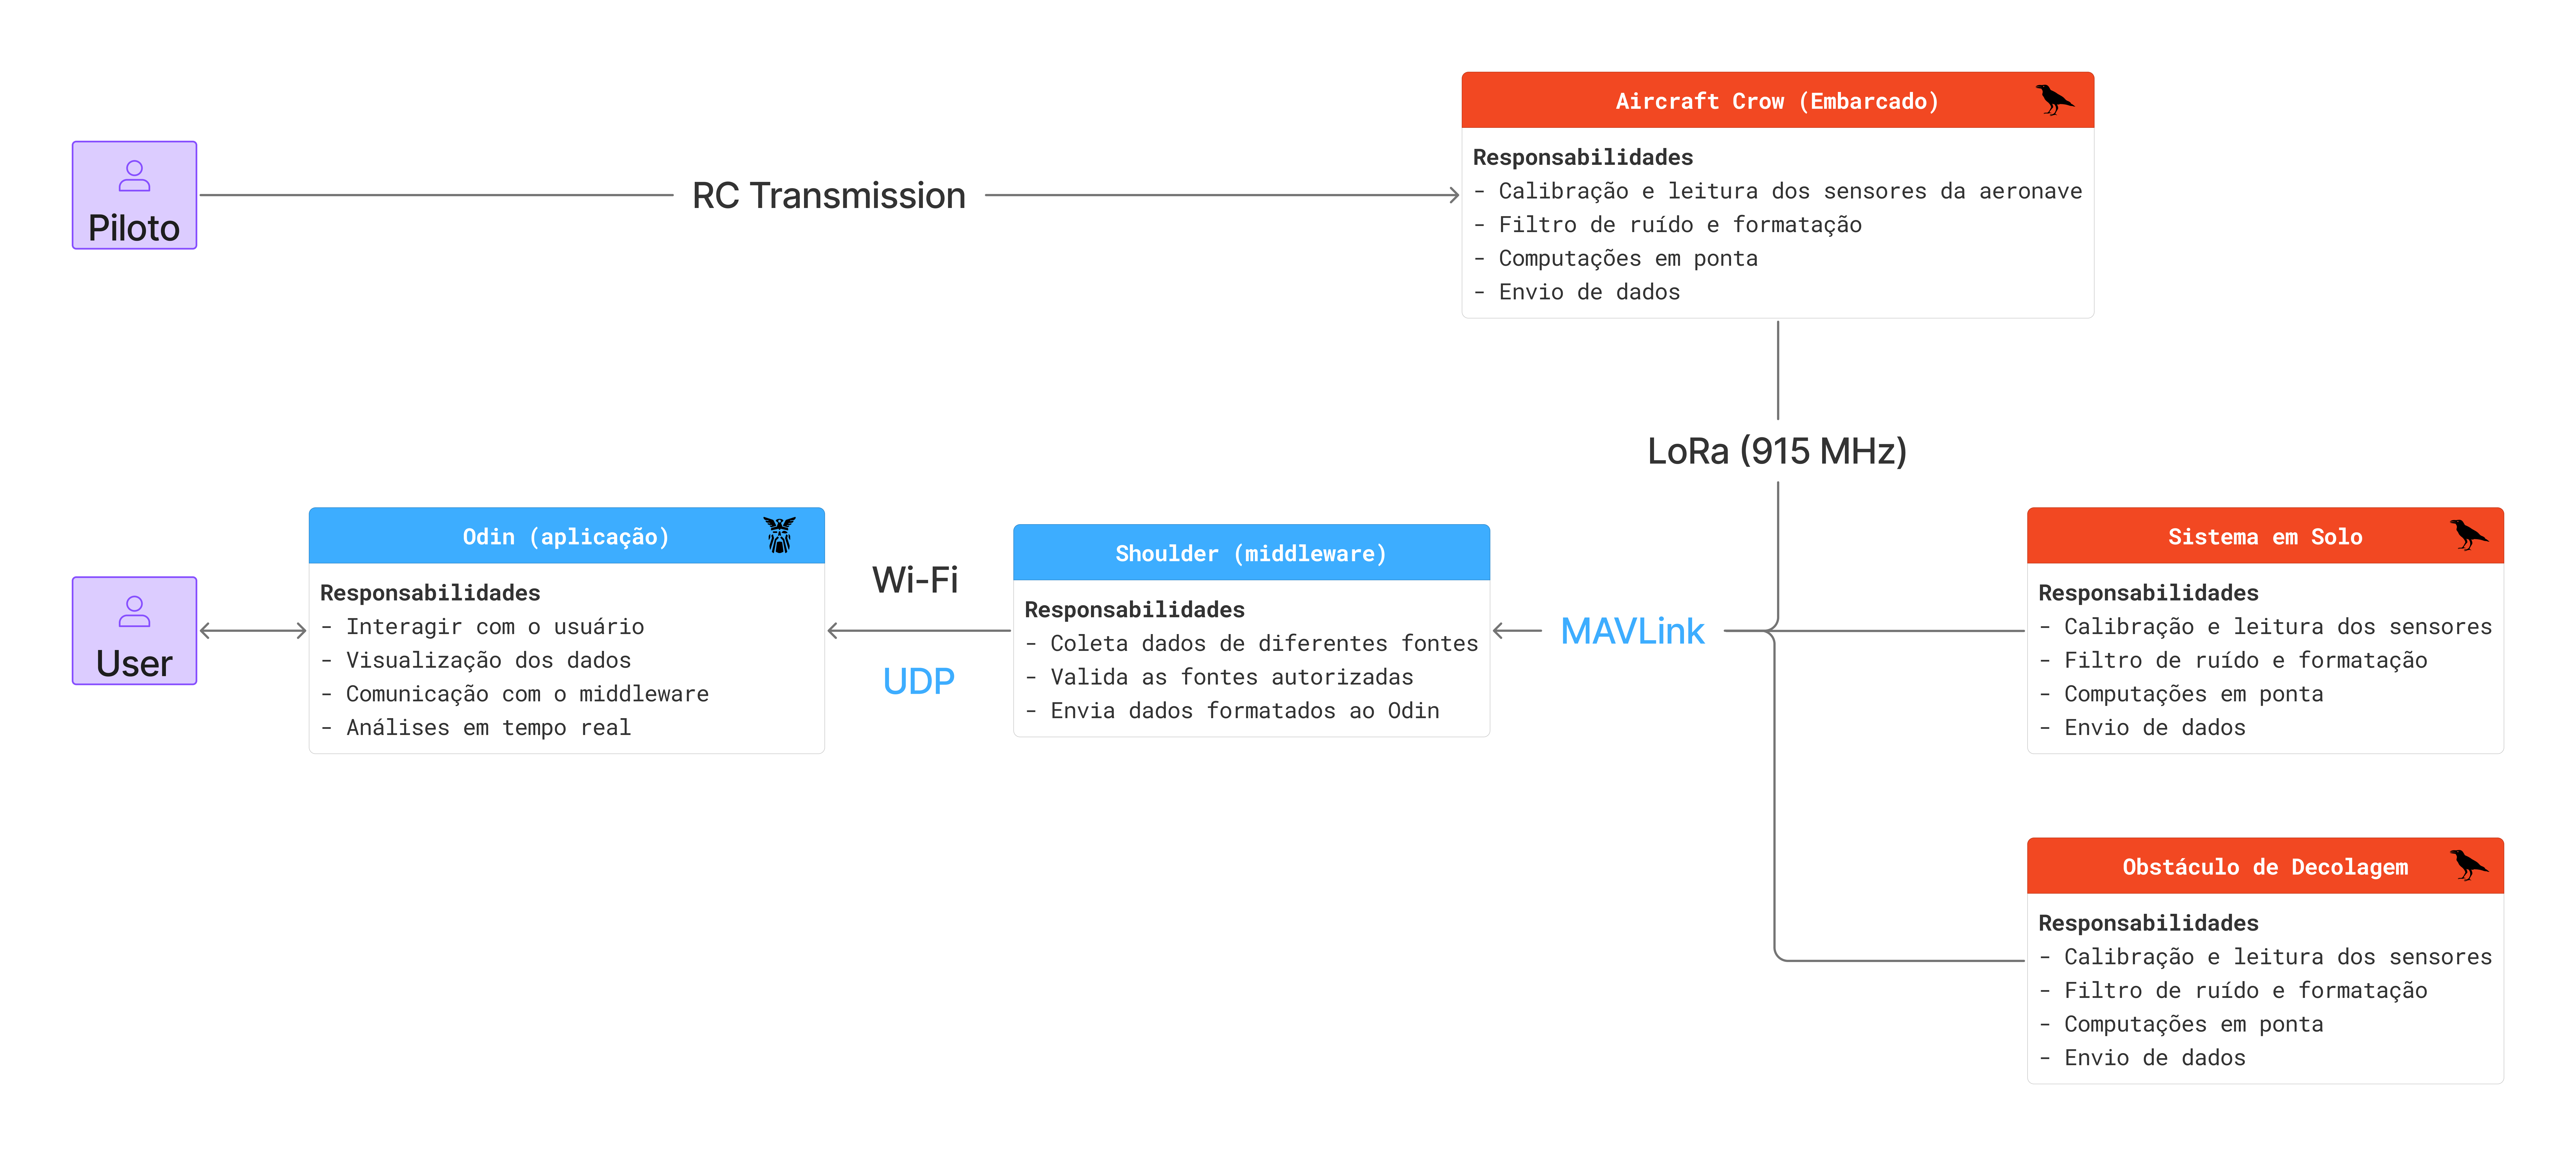
\includegraphics[width=0.85\textwidth]{images/design_de_comunicacao.png}
    \caption{\textit{Design} de comunicação}
    \label{fig:design-de-comunicacao}
\end{figure}


	\chapter{Sistema Embarcado}
\label{cap:sistema-embarcado}

\section{Casos de Uso}
Descrição de cada caso de uso e como o usuário irá interagir com o sistema

\section{Microcontrolador}
A escolha da unidade de processamento central é um dos pilares para o desenvolvimento deste componente, visto que o microcontrolador deve balancear restrições físicas e elétricas com a demanda por processamento de dados em tempo real. Desta forma, realizou-se uma comparação entre duas principais arquiteturas concorrentes no cenário de sistemas distribuídos embarcados: o microcontrolador Espressif ESP32 e o STMicroelectronics STM32F405RG.

O dimensionamento da topologia de alimentação elétrica do sistema é diretamente impactado pelas características de consumo do circuito integrado. A arquitetura Xtensa do ESP32 demonstra um consumo energético mais elevado. Mesmo quando os módulos de radiofrequência nativos (Wi-Fi e Bluetooth) são completamente desativados via \textit{software}, o núcleo consome continuamente entre 30 mA e 50 mA apenas para a manutenção do agendador do sistema operacional de tempo real (FreeRTOS) em estado de ociosidade \cite{esp32_datasheet}. 

Quando associado aos picos transientes de corrente demandados pela transmissão de longo alcance via rádio, este comportamento impõe a necessidade de uma arquitetura de regulação de tensão mais complexa com conversores chaveados e capacitores baixa resistência em série equivalente (ESR) para mitigar quedas abruptas de tensão e instabilidades térmicas na placa.

Em contrapartida, a arquitetura ARM Cortex-M4 presente no STM32F405RG foi projetada sob o paradigma de eficiência para baixo consumo. Operando em sua frequência máxima de 168 MHz, o dispositivo apresenta um consumo dinâmico previsível situado na faixa de 30 mA a 40 mA, mantendo uma dissipação térmica estável e eliminando a exigência de malhas complexas de alívio térmico ou dissipadores na placa-base. \cite{STM32F405RG_datasheet}

O ESP32 apresenta elevada capacidade de processamento por meio de sua arquitetura \textit{Dual-Core} com dois núcleos operando a 240 MHz (Xtensa LX6). Esta característica possibilita o isolamento completo de tarefas através do escalonamento simétrico, alocando o processamento de baixo nível e a leitura de sensores em barramentos I2C/SPI ao Core 0, enquanto o gerenciamento da máquina de estados (FSM) e o orquestrador principal executam no Core 1. Essa separação impede que as latências de escrita de arquivos em cartões de memória provoquem perda de amostras de dados. No entanto, o seu coprocessador de ponto flutuante é menos otimizado e a arquitetura de cache do FreeRTOS introduz pequenas variações de latência (\textit{jitters}).

Por outro lado, o STM32F405RG adota um único núcleo operando a 168 MHz, porém integra uma Unidade de Ponto Flutuante (FPU) nativa implementada diretamente por \textit{hardware} \cite{STM32F405RG_datasheet}. Durante o cálculo de filtros matemáticos complexos, a FPU executa as operações de ponto flutuante de forma quase instantânea. Ademais, a arquitetura ARM fornece um determinismo de \textit{hardware} em tempo real superior, assegurando que interrupções críticas associadas aos sensores sejam atendidas com latências fixas e previsíveis.

A integração física e lógica com múltiplos periféricos síncronos e assíncronos requer controladores de barramento robustos e isolados de ruído. O ESP32 emprega uma matriz de comutação de GPIO altamente flexível, permitindo o mapeamento de pinos lógicos I2C, SPI e UART para praticamente qualquer terminal físico do encapsulamento, o que simplifica o desenvolvimento do \textit{layout} de trilhas da placa de circuito. Contudo, os controladores internos de barramento da família Espressif historicamente apresentam limitações e anomalias de comportamento em silício sob condições de alta carga de dados, exigindo rotinas complexas de tratamento de exceções no \textit{software} para evitar travamentos do barramento em caso de falhas de sincronismo de um sensor \cite{esp32_gpio_anomalies}.

Já o STM32F405RG conta com periféricos de comunicação dedicados com posições de pinos imutáveis. Seus controladores I2C, SPI e USART são blindados internamente em \textit{hardware}, apresentando maior imunidade a ruídos. Adicionalmente, o dispositivo dispõe de um barramento nativo de entrada e saída digital segura (SDIO) por \textit{hardware} \cite{STM32F405RG_datasheet}. A gravação e a persistência de registros de voo através de uma interface SDIO dedicada alcança taxas de transferência substancialmente superiores e com maior confiabilidade do que a emulação de cartões através do protocolo SPI genérico tipicamente implementada em plataformas baseadas no ESP32.

A análise indica que, para o cenário deste sistema, desprovido da necessidade de conectividade sem fio de curto alcance nativa, o ecossistema STM32 alinha-se melhor aos requisitos de determinismo, tolerância a falhas e confiabilidade exigidos.

Contudo, apesar das vantagens de \textit{hardware} apresentadas pela plataforma ARM, o microcontrolador ESP32 foi selecionado para a implementação final do protótipo deste trabalho devido à viabilidade de execução, destacando-se na ampla acessibilidade local aos componentes e módulos de desenvolvimento, no menor custo relativo de instrumentação e na robustez das cadeias de suprimentos disponíveis, garantindo o cumprimento dos prazos.

Com esta decisão, iniciou-se o processo de desenho do esquemático do circuito eletrônico, representado com o microcontrolador na Imagem \ref{fig:mc_scheme}. Vale citar que, para melhor manutenção, simplicidade e devido a motivos de acessibilidade, o sistema será implementado a nível de módulos comerciais. Ou seja, os componentes serão todos \textit{Through-hole technology} (THT) soldados a uma placa caseira com trilhas em cobre.

\begin{figure}[ht]
    \centering
    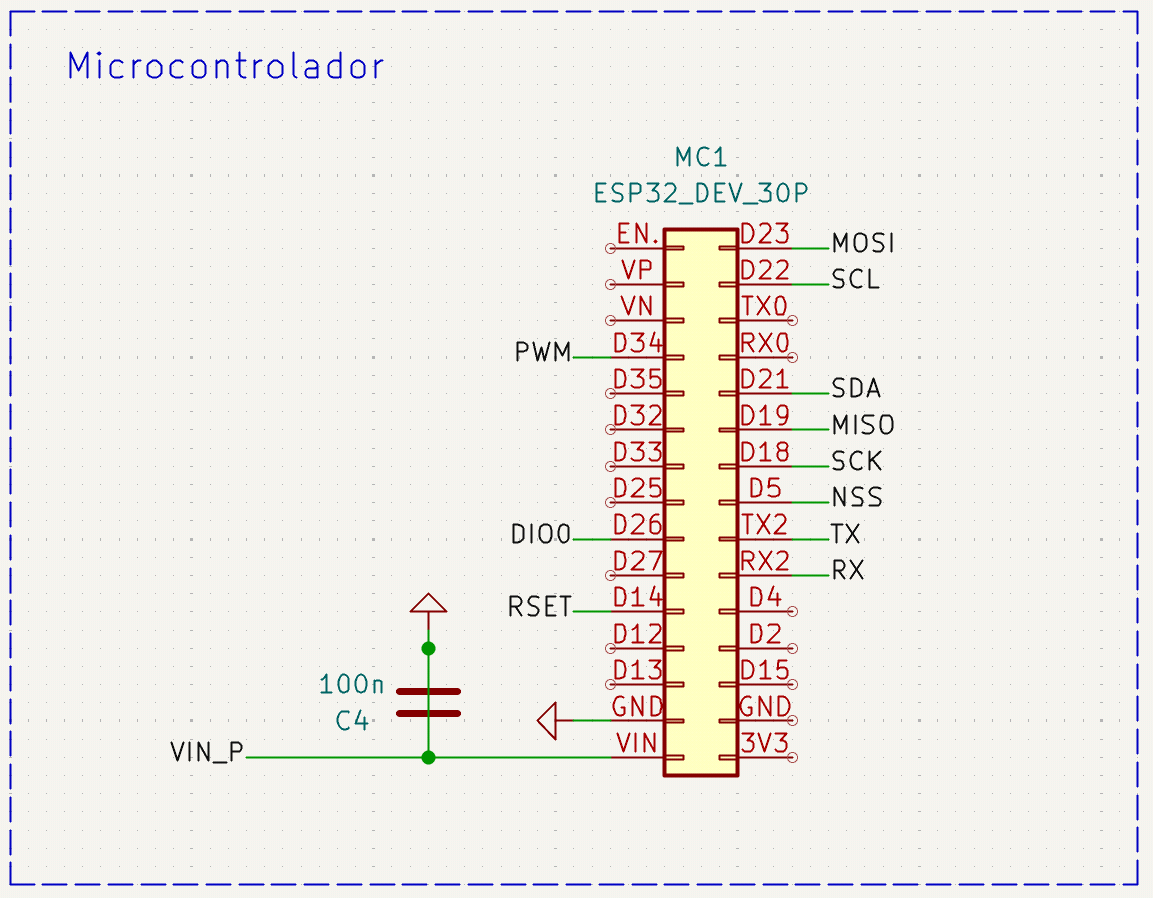
\includegraphics[width=0.9\textwidth]{images/mc_scheme.png}
    \caption{Esquemático Microcontrolador} \label{fig:mc_scheme}
\end{figure}

Por fim, para amenizar possíveis quedas de tensão em momentos de alta demanda da corrente, anexou-se um capacitor cerâmico de $100 nf$ em paralelo com a entrada VIN do ESP32. Por mais que módulos comerciais como o ESP32 Dev Kit já tenham sistemas integrados de controle energético, é importante garantir que não haja renícios forçados por subtensão (\textit{brownout}).

\section{Sensores e Módulos}
A seleção dos módulos de aquisição do sistema embarcado foi especificamente motivada pelos requisitos funcionais de telemetria. Conforme estabelecido previamente na Tabela \ref{tab:dados-requisitados}, o hardware em nível físico deve ser capaz de prover a aceleração no eixo da gravidade, a atitude espacial da aeronave, a velocidade relativa ao solo e a razão de subida da aeronave. Para satisfazer simultaneamente o escopo analítico das equipes de Cargas, Desempenho e Estabilidade, o sistema de aquisição deve consolidar componentes que operem sob margens de confiabilidade, lidando com os ruídos mecânicos e elétricos característicos do ambiente de voo.

Para o fornecimento dos dados de atitude tridimensional e do vetor de aceleração da gravidade, o projeto exige a implementação de um Sistema de Referência de Atitude e Proa (AHRS). Em ciclos de desenvolvimento passados, componentes de 6 graus de liberdade (6-DOF), a exemplo do legado MPU6050, figuraram como escolhas padrão \cite{tinyml_flight_phases}. Contudo, a ausência de um magnetômetro integrado neste encapsulamento impede a correção do vetor magnético terrestre, resultando na acumulação progressiva de erro matemático (\textit{drift}) no eixo de guinada. 

Outra alternativa amplamente adotada na instrumentação de baixo custo é o sensor BNO055, que integra 9 eixos e um coprocessador para fusão sensorial em hardware \cite{BNO055_datasheet}. Embora essa solução reduza drasticamente o esforço computacional do microcontrolador, sua arquitetura fechada impede a aplicação de filtros customizados e a escolha do componente onde a atitude será inferida, forçando o sistema a enviar pacotes maiores pela rede LoRa.

Desta forma, o presente sistema adota o módulo ICM-20948 como Unidade de Medição Inercial (IMU) primária. Trata-se de uma arquitetura de 9 eixos (acelerômetro, giroscópio e bússola) que entrega dados brutos de boa fidelidade. A associação física do magnetômetro ao silício, somada ao baixo perfil de ruído térmico e mecânico reportado pelo fabricante, confere ao barramento de comunicação uma amostragem satisfatoriamente limpa \cite{ICM-20948_datasheet}.

As análises conduzidas pelo subsistema de Desempenho e a validação do envelope de voo pelo subsistema de Cargas requerem a coleta de dados de translação aerodinâmica e referencial de pista. A aferição da velocidade relativa ao solo é atendida pela integração de um módulo receptor de Sistemas Globais de Navegação por Satélite (GNSS). Módulos legados, como o NEO-6M, limitam-se ao rastreamento primário da constelação GPS com taxas de atualização de apenas 1 Hz a 5 Hz \cite{NEO-6M_datasheet}, induzindo uma latência inaceitável para a dinâmica de manobras das aeronaves. Portanto, selecionou-se o receptor NEO-8M, que suporta o rastreio simultâneo de múltiplas constelações (GPS, GLONASS, Galileo) e fornece atualizações em frequências de até 10 Hz, assegurando a confiabilidade, a precisão posicional e o sincronismo temporal dos vetores de velocidade \cite{NEO-8M_datasheet}.

Por fim, a derivação da razão de subida e a correção da leitura altimétrica fornecida pelo GNSS demandam o monitoramento da pressão atmosférica estática. Soluções comerciais genéricas voltadas para a Internet das Coisas (IoT), como o BMP280, apresentam um piso de ruído e uma variação de medida que comprometem a precisão da aquisição \cite{BMP280_datasheet}. Portanto, adotou-se o módulo MS5611, que fornece uma resolução altimétrica efetiva na escala de centímetros \cite{MS5611_datasheet}. Essa informação é então utilizada para atenuar as margens de erro intrínsecas ao posicionamento por satélite no eixo vertical.

TODO: Tabelas comparativa

Os \textit{footprints} dos componentes comerciais foram desenhados conforme os \textit{datasheets} de cada módulo. Além disso, os sensores foram adicionados ao esquema de circuito do hardware, apresentado na Imagem \ref{fig:sensor_scheme}.

\begin{figure}[ht]
    \centering
    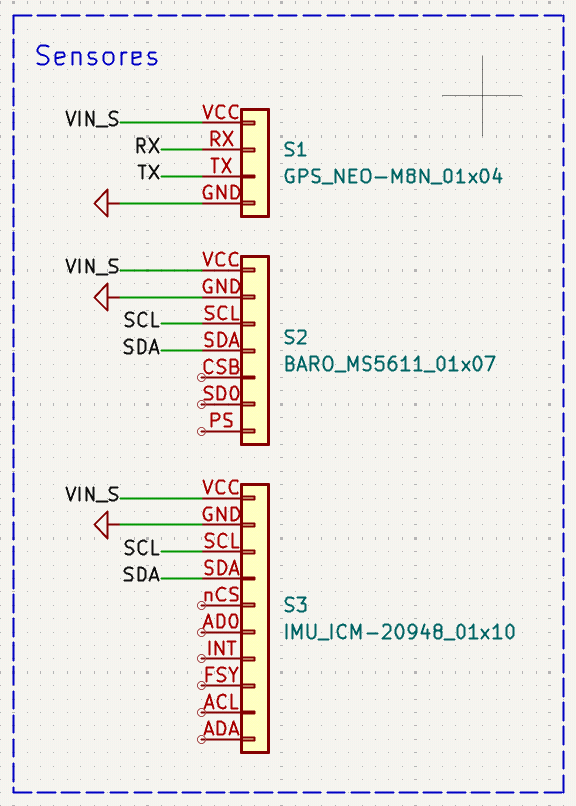
\includegraphics[width=0.55\textwidth]{images/sensors_scheme.png}
    \caption{Esquemático dos Sensores} \label{fig:sensor_scheme}
\end{figure}

Com os sensores determinados e os protocolos seriais identificados, seguiu-se para o próximo passo de determinar os componentes de comunicação. Estes, serão também módulos comerciais, porém com outro escopo de decisão e implementação.

\section{Componentes de Comunicação}
Para este sistema, existem três componentes de comunicação: o módulo de transmissão LoRa, a interface PWM com o receptor da aeronave e um \textit{buzzer} ativo para alertas sonoros.

Para a interface PWM, a necessidade é de apenas um barramento para o sinal modular e um barramento para compartilhamento do GND. Visando valorizar a integração da placa com o sistema de controle existente, utilizou-se de um trio de cabos AWG 24 com conctores fêmeas. Esse trio comumente abrange o sinal, o terra e o positivo.

Aqui, surge a oportunidade de ligar o sistema embarcado no mesmo sistema de alimentação do sistema de controle, aproveitando da bateria e componentes já existentes. Esta possibilidade será melhor discutida mais à frente no texto.

Para o módulo LoRa, a principal restrição se dá pelas normas de frequências permitidas para operação \cite{norma_frequencias}. Das opções comercialmente disponíveis, a única variação permitida para operação livre no Brasil é a de frequência $915 MHz$. 

Além disso, o acesso aos módulos pode ser relativamente custoso financeiramente. Portanto, a comparação entre os principais módulos que atendem ao requisito de frequência permitida se deu pelo valor e compatibilidade com o microcontrolador escolhido, como visto na Tabela \ref{tab:modulos_lora}.

Dessa forma, o módulo escolhido foi o SX1276, sendo a Figura \ref{fig:comm_scheme} a adição do LoRa, do PWM e do \textit{buzzer} ao esquemático do projeto.

\begin{figure}[ht]
    \centering
    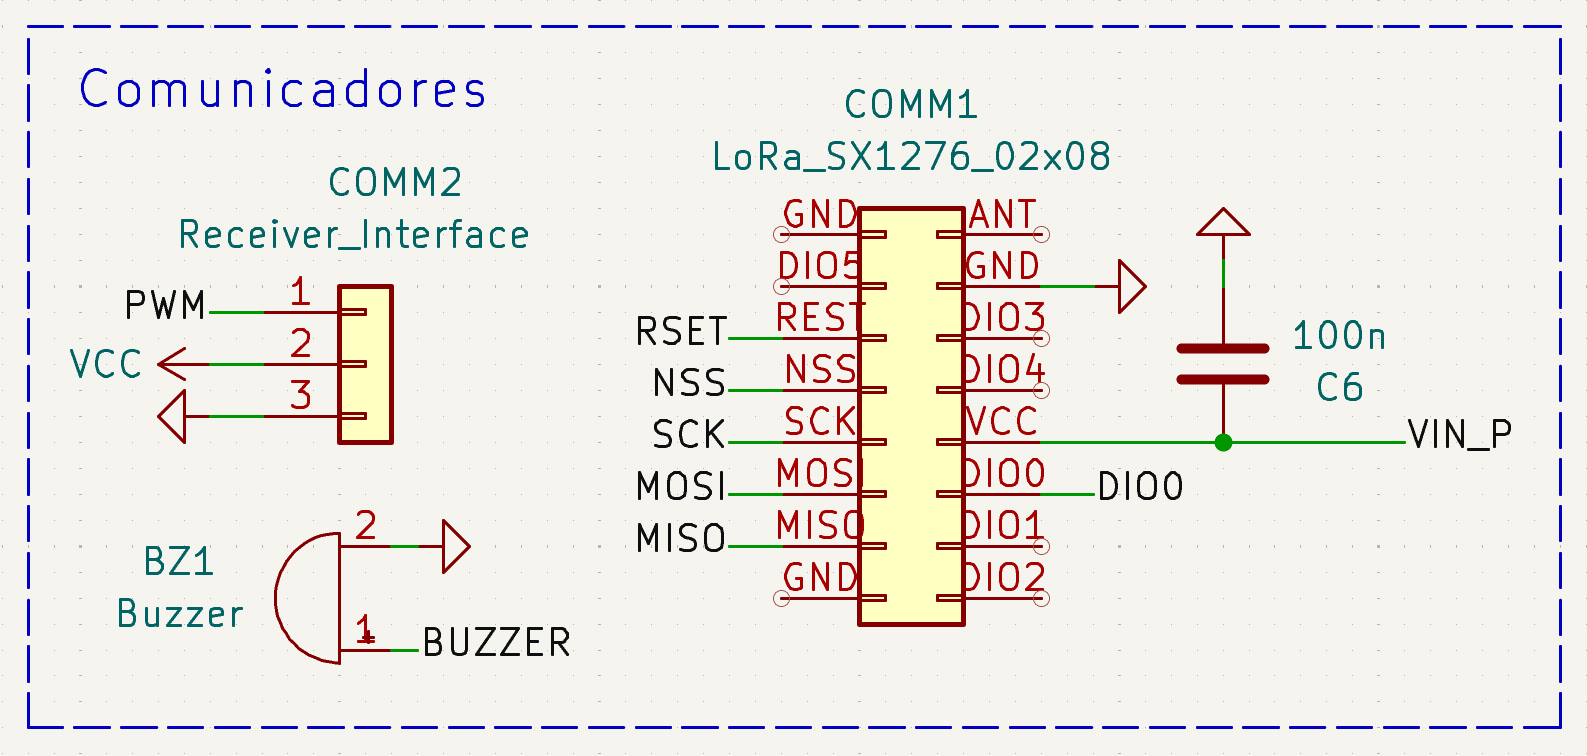
\includegraphics[width=0.9\textwidth]{images/comm_scheme.png}
    \caption{Esquemático dos Comunicadores} \label{fig:comm_scheme}
\end{figure}

Por fim, vale citar que o módulo LoRa SX1276 exige correntes de pico consideráveis --característica intrínseca dos transmissores de alto alcance --, aproximando-se de $120 mA$ quando configurado para transmitir na potência máxima de $+20 dBm$ \cite{SX1276_datasheet}. Por isso, adicionou-se um capacitor de $100 nf$ em paralelo à entrada VCC do módulo, criando um amortecimento aos picos de potência que o LoRa irá provocar. O pico de consumo do SX1276 não é um fator bloqueante, mas se torna um ponto de atenção para o dimensionamento da camada de alimentação energética do sistema.

\section{Rede de Distribuição de Potência e Dimensionamento Elétrico}
O projeto de hardware para um sistemas aviônicos embarcado planejamento criterioso da rede de distribuição de potência (PDN). Em VANTs, as oscilações elétricas induzidas por atuadores mecânicos do sistema de controle e as restrições de dissipação térmica representam desafios para a estabilidade do microcontrolador e componentes.

\subsection{Definição da Fonte e Levantamento de Carga}
O subsistema embarcado recebe energia diretamente dos pinos de barramento do receptor de rádio acoplado ao sistema de controle da aeronave. Esse barramento é alimentado por uma bateria de fosfato de ferro-lítio (LiFePO4) de duas células (2S), que apresenta uma tensão nominal de $6,6 V$, podendo atingir $7,2 V$ quando em estado de carga máxima \cite{LiFePO4}.

Para o dimensionamento físico da rede elétrica, realizou-se um levantamento da demanda de corrente do hardware em regime de operação. O microcontrolador base terá um consumo típico estabilizado, mas demandará correntes complementares durante as rotinas de inicialização \cite{esp32_datasheet}. Simultaneamente, o módulo LoRa operando na banda de $915 MHz$ exige uma demanda instantânea de corrente de aproximadamente $120 mA$ durante os ciclos de transmissão em potência máxima de $+20 dBm$ \cite{SX1276_datasheet}. Estima-se que, sob condições normais de operação, o pico de consumo total do arranjo de processamento, sensores e rádio situa-se em aproximadamente $700 mA$.

\subsection{Problemática Térmica e Ruído Conduzido}

A imposição de rebaixar o nível de tensão de até $7,2 V$ para o patamar operacional de $3,3 V$ sob uma corrente contínua de $0,7 A$ introduz a necessidade de atenção às restrições térmicas. Caso a arquitetura adotasse uma regulação estritamente linear por meio de componentes monolíticos padrão — como o regulador AMS1117-3.3 —, a potência dissipada exclusivamente sob a forma de calor ($P_D$) seria calculada pela Lei de Joule:

$$P_D = (V_{in} - V_{out}) \cdot I$$
$$P_D = (7,2\text{ V} - 3,3\text{ V}) \cdot 0,7\text{ A} = 2,73\text{ W}$$

Considerando que o encapsulamento físico desses reguladores lineares suporta um limite prático de dissipação térmica próximo a $1,0 W$ em ambientes fechados, a exigência de $2,73 W$ sobrecarregaria o componente em poucos segundos. Esse excesso de calor ativaria os circuitos internos de proteção térmica, resultando no desligamento completo do sistema de telemetria durante o voo \cite{thermal_management}.

Além da restrição térmica, o barramento elétrico é compartilhado com os servomotores da aeronave por meio do receptor. O acionamento dinâmico dessas cargas indutivas gera picos de força contraeletromotriz e quedas severas na tensão de entrada. Sem o devido isolamento elétrico, os disparos rápidos de transmissão do módulo LoRa provocam quedas localizadas de voltagem, colocando o microcontrolador em um estado de \textit{brownout} \cite{the_art_of_electronics}.

\subsection{Arquitetura de Distribuição de Energia \textit{Dual-Rail}}

Para contornar as limitações térmicas e isolar os ruídos conduzidos, implementou-se uma topologia de alimentação do tipo \textit{Dual-Rail}, distribuindo a energia em duas vias independentes:

\begin{itemize}
  \item{\textbf{Trilha de Potência:} Direcionada aos componentes de consumo elevado e perfil ruidoso, nominalmente o microcontrolador e o transceptor de rádio. Utiliza-se o mini-360, um conversor \textit{Step-Down} chaveado que reduz a tensão de entrada para $3,3 V$ com eficiência superior a $85\%$. Esse módulo suporta picos de corrente de até $2 A$ sem gerar dissipação térmica expressiva, garantindo a estabilidade operacional dos módulos de comunicação \cite{mini360_datasheet}.}
  \item{\textbf{Trilha Sensível:} Dedicada exclusivamente aos componentes de instrumentação (IMU, barômetro e GNSS), cujo consumo somado é baixo. Um regulador linear de baixa queda de tensão (LDO), alimentado diretamente pela fonte primária, fornece uma saída isolada em $3,3 V$. Devido à baixa corrente dos sensores, o calor gerado é mínimo. A vantagem desta abordagem reside na pureza espectral do sinal elétrico, visto que os LDOs barram os ruídos de alta frequência provenientes do chaveamento do conversor \textit{Buck} e das transmissões de rádio, preservando a integridade das leituras analógicas e digitais dos sensores \cite{power_delivery_network_design}.}
\end{itemize}

\subsection{Dimensionamento de Filtros e Análise de Transientes}

Para garantir o amortecimento dos transientes de carga e prevenir oscilações que violem os limites operacionais dos circuitos integrados, o dimensionamento dos capacitores de desacoplamento e armazenamento local baseou-se na equação fundamental da capacitância em função da variação temporal de corrente e tensão:

$$C = I \cdot \frac{\Delta t}{\Delta V}$$

No nó de transmissão de $3,3 V$ (compartilhado pelo processador e pelo rádio), estima-se que o degrau de corrente abrupto ($I$) atinja $0,62 A$ durante as janelas de calibração e envio de pacotes. Sabendo que o limite inferior de integridade dos circuitos de radiofrequência ocorre em $3,0 V$, a queda de tensão máxima tolerável ($\Delta V$) no barramento é de $3,3\text{ V} - 3,0\text{ V} = 0,3\text{ V}$. Assumindo um tempo de resposta aproximado ($\Delta t$) de $200\,\mu\text{s}$ para que a malha de realimentação do conversor \textit{Buck} compense a demanda repentina \cite{mini360_datasheet}, o cálculo da capacitância necessária resulta em:

$$C = 0,62\text{ A} \cdot \frac{0,0002\text{ s}}{0,3\text{ V}} \approx 413\,\mu\text{F}$$

Para suprir essa demanda com margem de segurança, adotou-se um capacitor eletrolítico de $470\,\mu\text{F}$ posicionado fisicamente próximo aos pinos de alimentação do circuito de controle. O componente selecionado apresenta uma resistência série equivalente de $150\text{ m}\Omega$ ($\text{ESR} = 0,15\,\Omega$) \cite{capacitor_esr}. Para mitigar a queda de tensão resultante dessa resistência e compensar a alta Indutância Série Equivalente (ESL) típica desse tipo de encapsulamento, adicionou-se um capacitor cerâmico de $100\text{ nF}$ em paralelo. Essa associação reduz a impedância total do conjunto em frequências elevadas, impedindo que flutuações de tensão indutivas ou resistivas reiniciem o processamento.

Na entrada primária de 6,6 V, o sistema deve suportar transientes mecânicos mais lentos gerados pelos servomotores, cujos distúrbios na linha de transmissão duram cerca de $1\text{ ms}$ ($\Delta t = 0,001\text{ s}$) \cite{servo_disturbio}. Considerando a corrente máxima de regime da placa de telemetria ($I = 0,7\text{ A}$) e estabelecendo uma margem de queda de tensão estritamente segura de $\Delta V = 1,0\text{ V}$ para manter a entrada dos reguladores acima do limite de \textit{dropout}, aplica-se a relação matemática:

$$C = 0,7\text{ A} \cdot \frac{0,001\text{ s}}{1,0\text{ V}} = 700\,\mu\text{F}$$

Visando trazer robustez ao hardware contra os altos consumos provenientes dos esforços nas superfícies de comando da aeronave, implementou-se um capacitor eletrolítico de $1000\,\mu\text{F}$ com isolação nominal de $16 V$ na entrada da placa. Em paralelo a esse componente, adicionou-se um capacitor cerâmico de $100\text{ nF}$ focado na supressão de ruídos de alta frequência induzidos pelos motores CC dos servos, completando a barreira de proteção eletromagnética do sistema embarcado \cite{electromagnetic_compatibility_engineering}.

Com a arquitetura idealizada, realizou-se a adição dos componentes ao esquemático da placa de circuito, conforme Imagem \ref{fig:power_scheme}

\begin{figure}[ht]
    \centering
    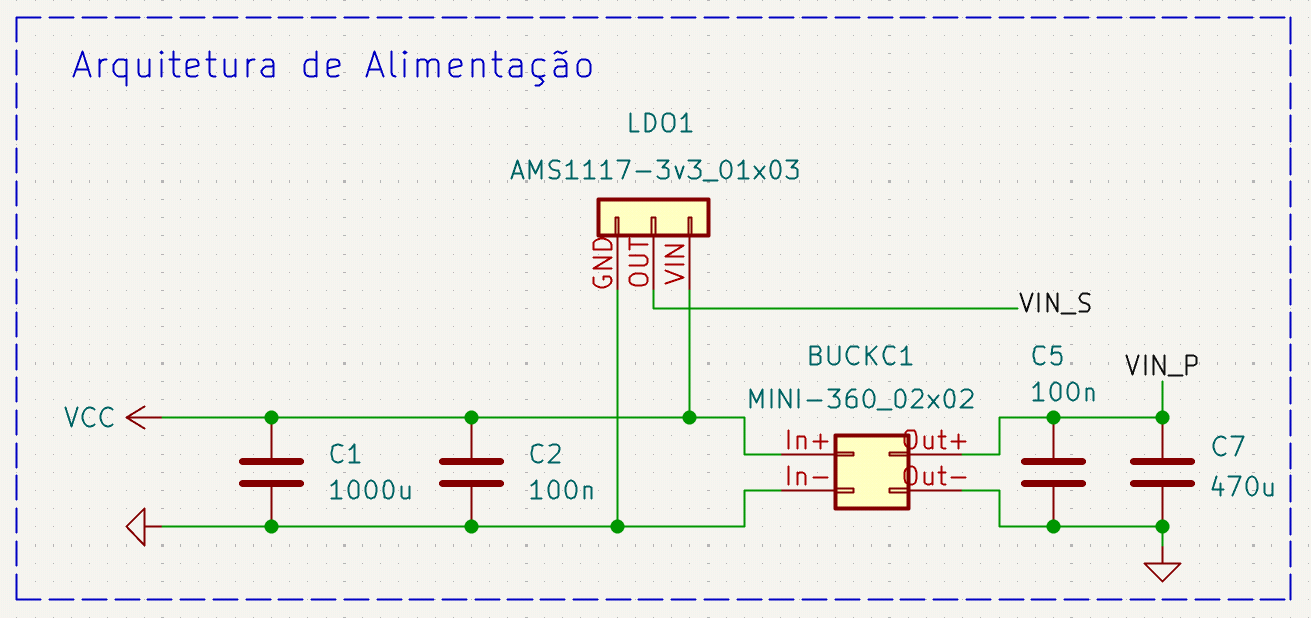
\includegraphics[width=0.9\textwidth]{images/power_scheme.png}
    \caption{Esquemático da Arquitetura de Alimentação} \label{fig:power_scheme}
\end{figure}

O desenho da arquitetura de alimentação marca o fim do processo de dimensionamento e escolha dos componentes eletrônicos. O esquemático apresentado é organizado de forma que facilite a leitura das conexões, mas não representa a disposição física dos componentes, nem o caminho exato das trilhas. Estas são funções do desenho da placa de circuito impresso (PCB), que procede o esquemático.

\section{Placa de Circuito Impresso}
Um dos maiores desafios no processo de fabricação de um sistema embarcado é a montagem do hardware. Existem algumas abordagens para esta etapa, podendo ser feita com placas de prototipagem (\textit{protoboards}), com placas cobreadas caseiras --como as placas de fenolite ou fibra de vidro laminadas com cobre--, ou ainda através da fabricação sob demanda em empresas especializadas em PCB.

Visto que o sistema irá ser embarcado em um VANT, a montagem em \textit{protoboards} está descartada. Para este projeto, será usado uma placa de fenolite duplamente cobreada, viabilizando vias nas duas faces da placa. Esta técnica é viável para produção caseira, mas exige cuidados no processo de desenho da PCB.

Os componentes podem ser adquiridos em dois níveis, conhecidos como \textit{Surface Mount Technology} (SMD) e \textit{Through Hole Technology} (THT). Placas feitas com SMD são mais compactas e com acabamento mais profissional, porém exigem a busca por distribuidores especializados que costumam vender apenas em grande quantidade. Além disso, a fabricação e manipulação de componentes SMT exigem ferramentas de precisão e prática especializada, que dificultaria e atrasaria o desenvolvimento do projeto.

Os componentes THT ocupam mais espaço e vêm prontos pra uso. Estes são mais fáceis de ter acesso e mais baratos em pequena quantidade. Além disso, a fabricação é facilitada pelos pinos que aumentam a área de contato para aplicação de estanho no processo de soldagem. Dessa forma, os componentes utilizados para este trabalho serão todos THT, valorizando a facilidade de montagem e manutenção do sistema. 

\subsection{Posicionamento dos Componentes}
Como primeiro passo para o desenho da PCB, o posicionamento dos componentes foi realizado. Para faciltar o caminho das trilhas, cada subsistema foi alocado em um espaço da placa com o cuidado de manter os limites dentro da margem do requisito RNF.03. A disposição está representada na Imagem \ref{fig:pcb_componentes}

\begin{figure}[ht]
    \centering
    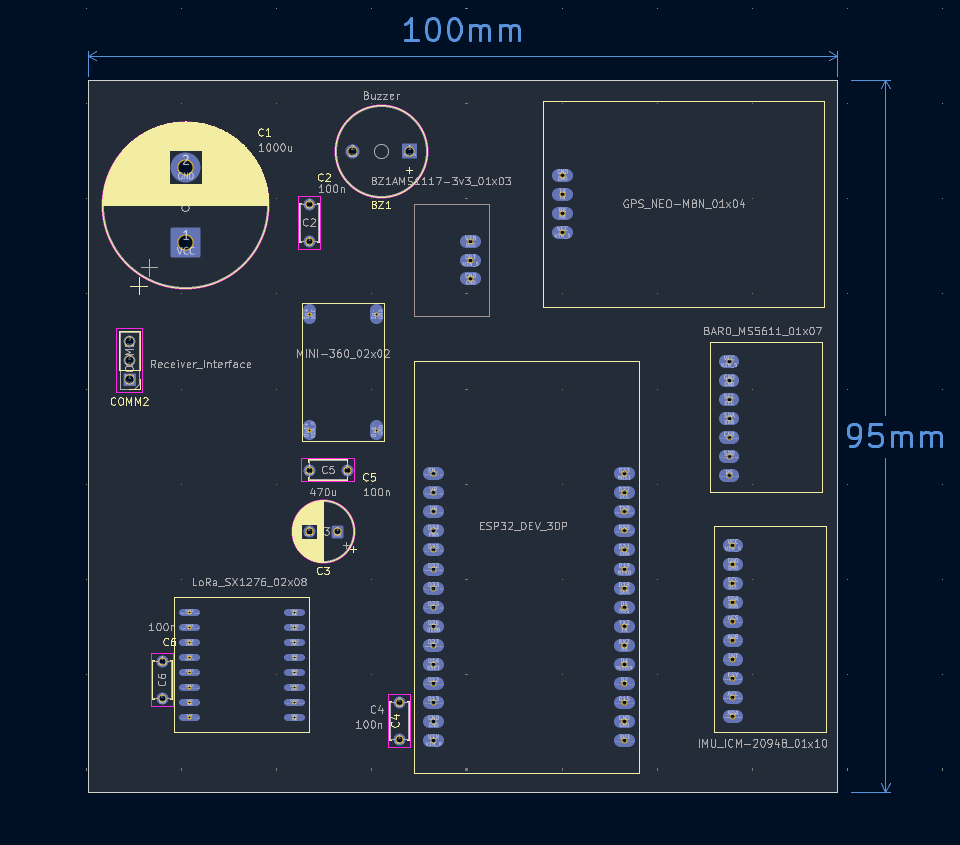
\includegraphics[width=0.8\textwidth]{images/pcb_componentes.png}
    \caption{Posicionamento dos Componentes na PCB} \label{fig:pcb_componentes}
\end{figure}

Com isso, o sistema de alimentação se concentrou ao lado esquerdo superior da face de cima da placa, com os capacitores de $100 nf$ posicionados próximo à entrada de cada componente. A entrada do PWM foi posicionada na extremidade para que o fio de acesso ao receptor comece para fora da placa. Já o SX1276 foi rotacionado de forma que sua antena fique na extremidade para facilitar a sua exposição no compartimento da aeronave.

Os sensores, ficaram ao lado contrário do sistema de alimentação para afastá-los das vias ruidosas de entrada.Em específico, o GPS foi alocado na extremidade superior direita para facilitar a integração da antena externa. Por fim, para garantir trilhas mais covenientes, o microcontrolador foi posicionado ao centro com o lado da entrada USB-C apontada para fora.

\subsection{Dimensionamento das Trilhas}
Antes de começar o desenho das trilha é importante determinar regras para garantir segurança no processo de manufatura, visto que será um processo manual. Dessa forma, determinou-se um padrão de $1 mm$ para todas as trilhas de informação e $1.8 mm$ para trilhas de alimentação. Além disso, para evitar contato entre trilhas determinou-se uma distância mínima de $0.6 mm$ entre qualquer trilha ou \textit{pad}. A partir destas regras, contruío-se as trilhas conforme Imagem \ref{fig:trilhas_pcb}, onde as trilhas vermelhas estão na face superior, e as trilhas azuis na face inferior.

\begin{figure}[ht]
    \centering
    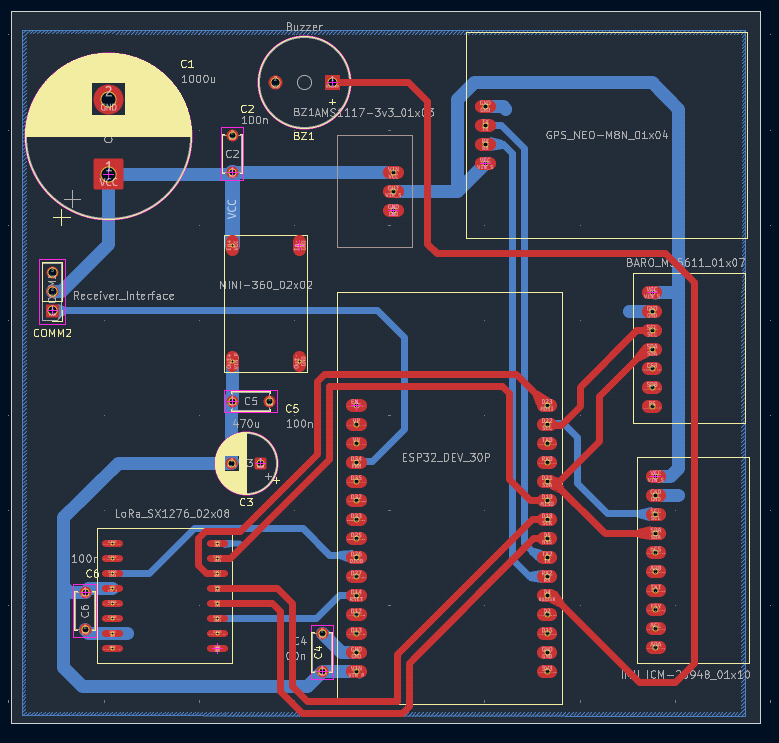
\includegraphics[width=0.8\textwidth]{images/trilhas_pcb.png}
    \caption{Disposição das Trilhas na PCB} \label{fig:trilhas_pcb}
\end{figure}

A maior parte das trilhas de informação foram posicionadas na face superior para que a face inferior fosse dedicada à zona preenchida e trilhas de alimentação. Além disso, aplicou-se o eforço de evitar trilhas com vias entre faces, ou seja, trilhas que usem as duas faces no mesmo percurso, diminuindo a complexidade construtiva da placa.

\subsection{Zona Preenchida (GND)}
Um prática comum em PCBs é a adição de uma zona preenchida para o GND. Esta estratégia cria um caminho de menor impedância para que a corrente retorne dos componentes, ajuda a proteger os sinais sensíveis de interferências eletromagnéticas, minimiza quedas de tensão, auxilia na distribuição de energia estável para todo o circuito, e ainda, reduz a quantidade de produto corrosivo no processo de corrosão da placa \cite{zona_preenchida}. Por isso, conforme Imagem \ref{fig:zona_gnd}, criou-se uma zona preenchida para o GND na face inferior da placa.

\begin{figure}[ht]
    \centering
    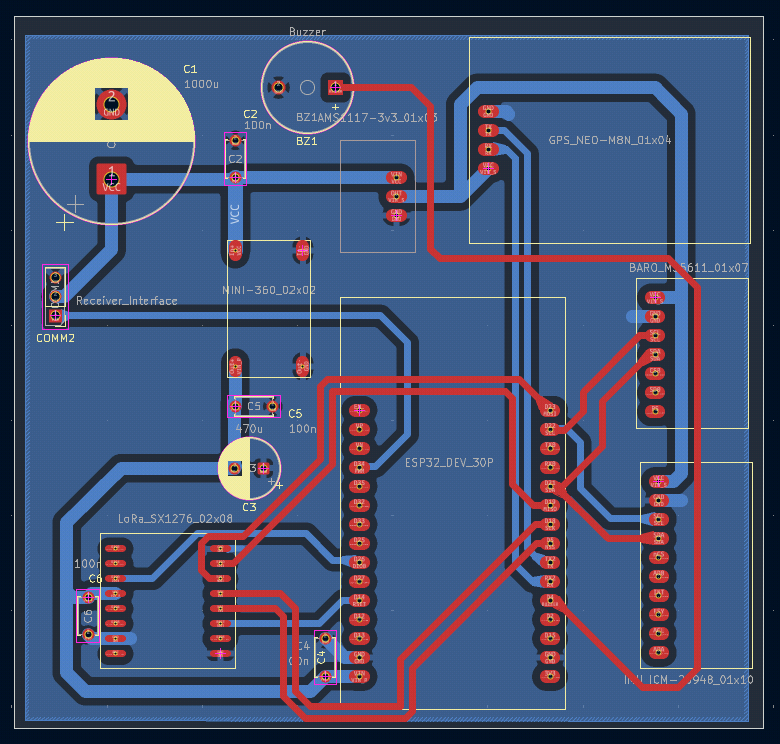
\includegraphics[width=0.8\textwidth]{images/zona_gnd.png}
    \caption{PCB com GND em Zona Preenchida} \label{fig:zona_gnd}
\end{figure}

Com isso, o desenho da PCB foi finalizado e enviado para impressão UV na placa de fenolite cobreada. Como forma de validação, conforme Imagem \ref{fig:pcb_a4} o circuito foi impresso em uma folha A4 para que os módulos pudessem ser fisicamente posicionados, validando a coerência do desenho com os componentes reais.

\begin{figure}[ht]
    \centering
    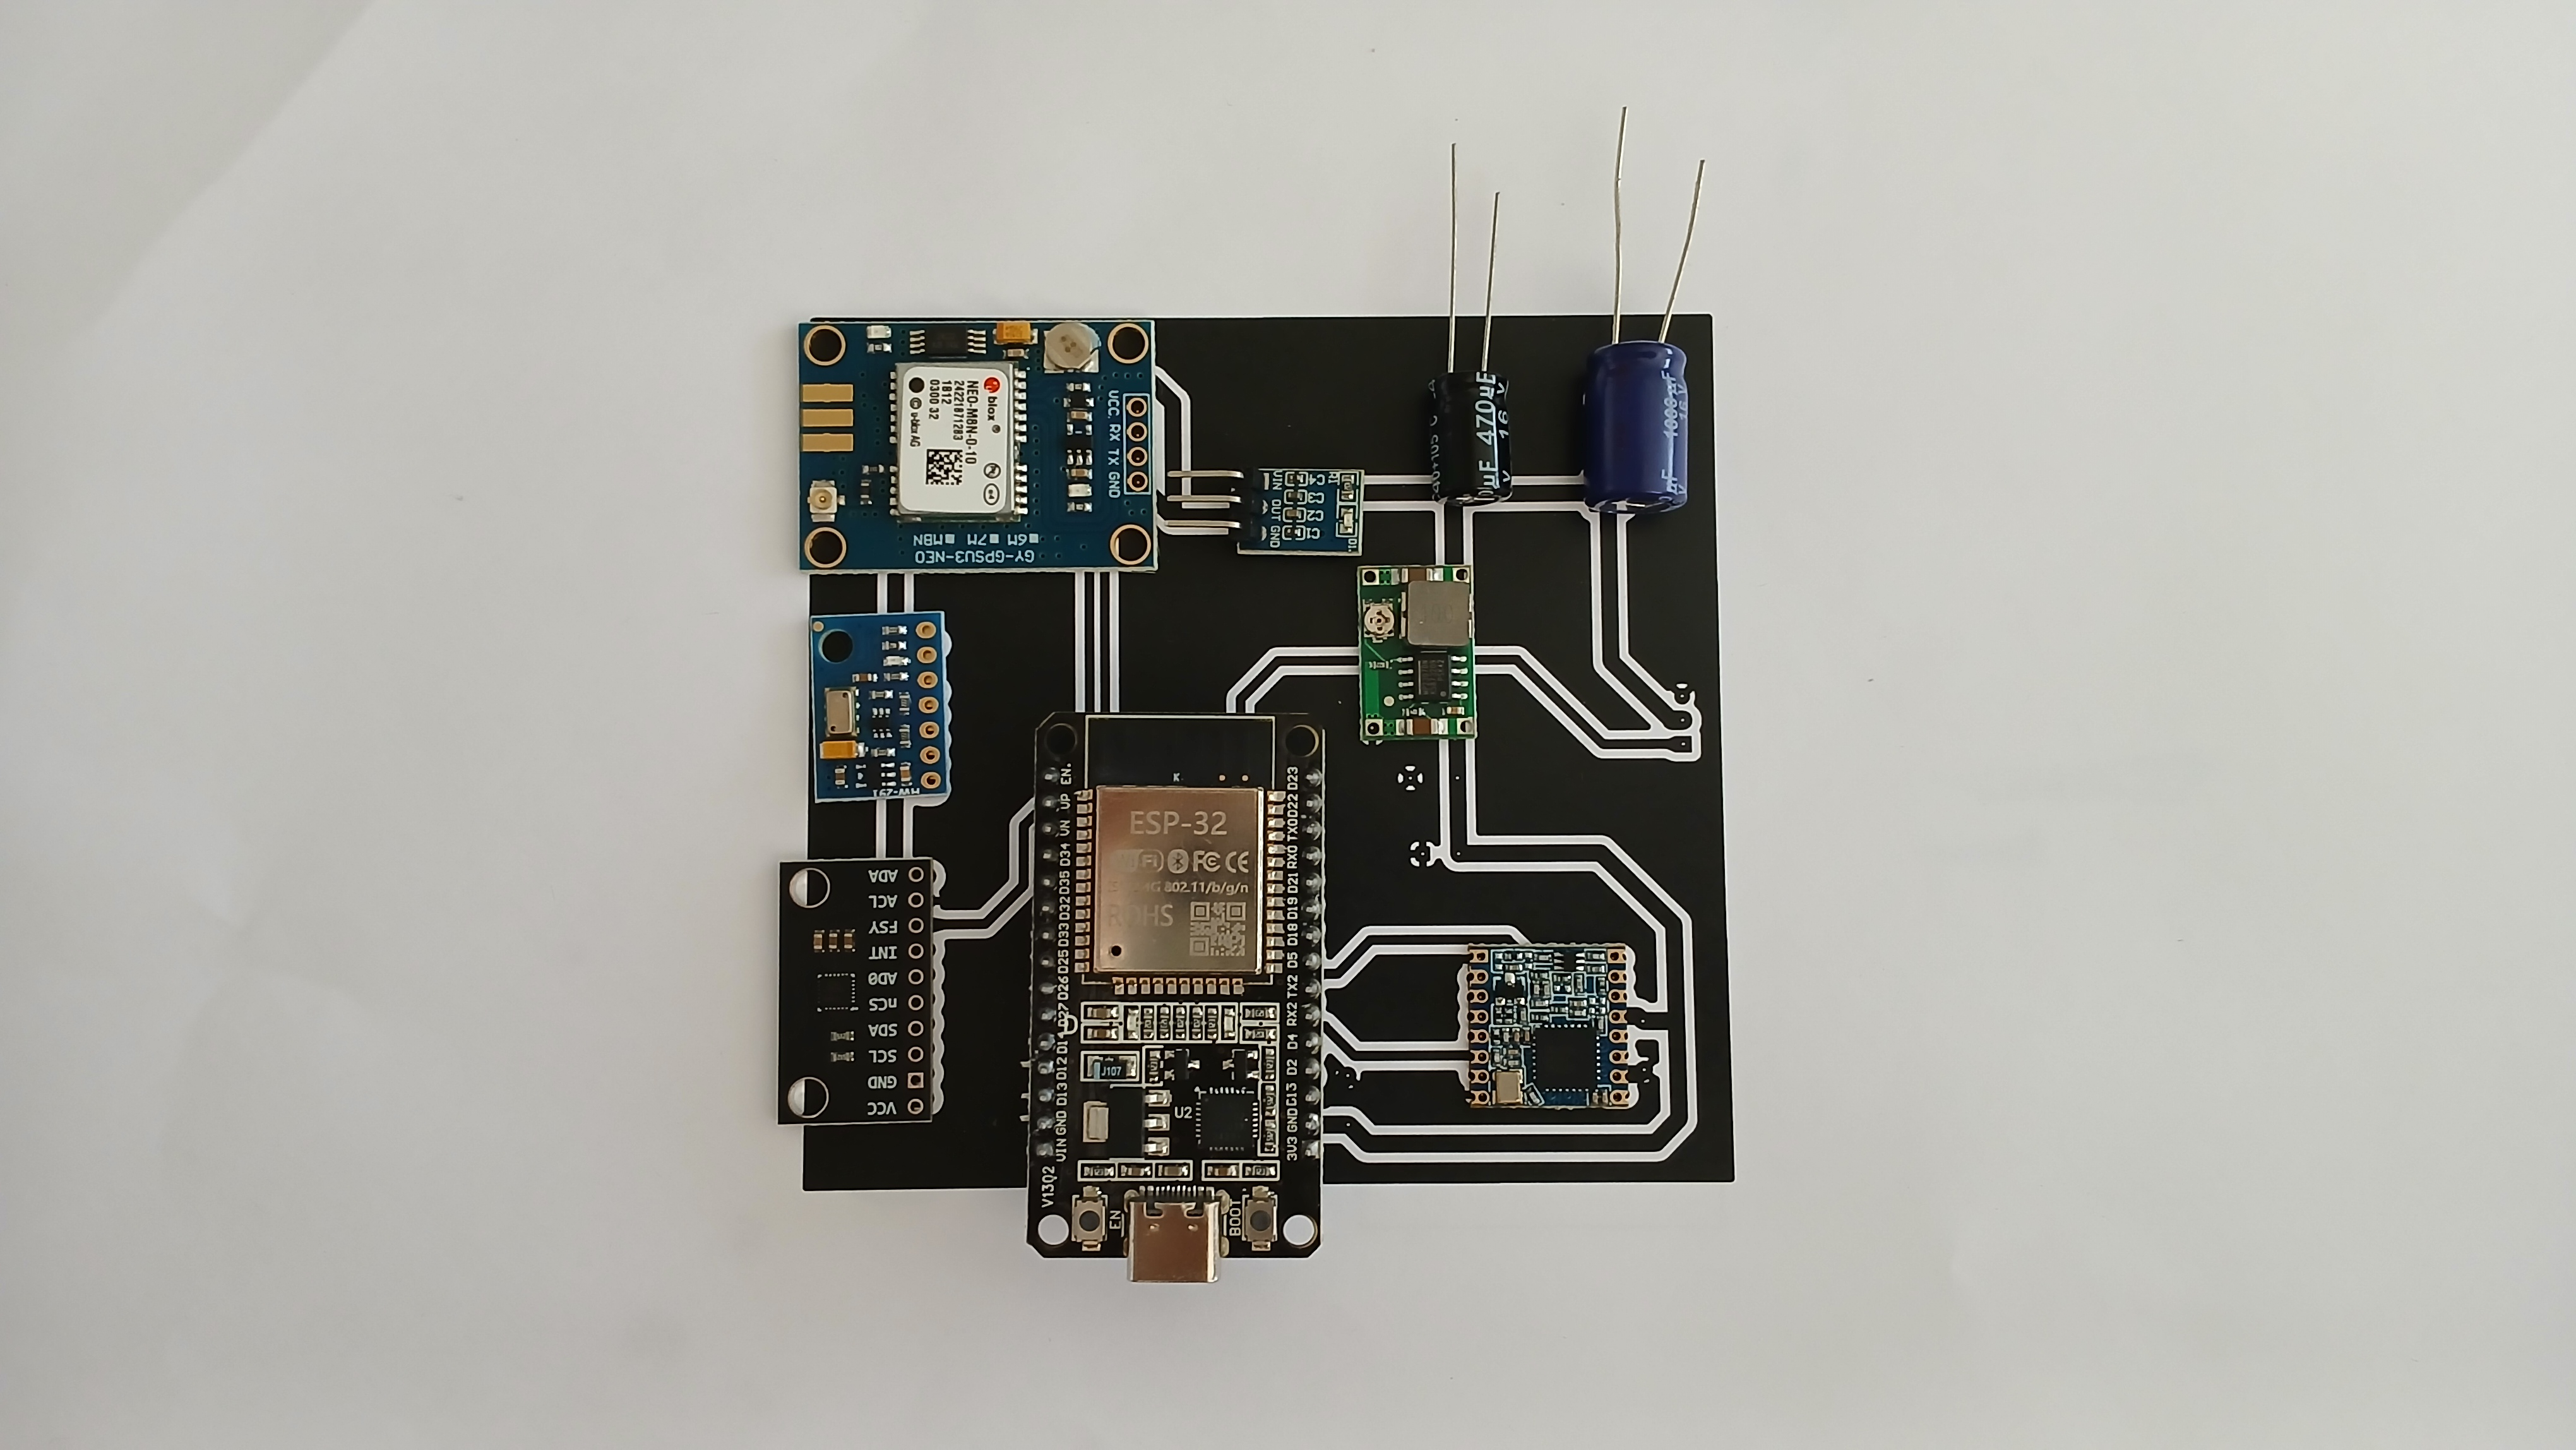
\includegraphics[width=0.9\textwidth]{images/pcb_a4.jpg}
    \caption{Validação do Posicionamento da PCB em Folha A4} \label{fig:pcb_a4}
\end{figure}

\section{\textit{Firmware}}
Para a implementação do \textit{Firmware} foram consideradas três vias de ferramentas. A primeira opção seria com programação \textit{bare-metal}, onde nenhuma camada de abstração externa é adicionada para dar total liberdade à implementação em baixíssimo nível de abstração \cite{software_embarcado}. Uma segunda alternativa é o uso de sistemas operacionais de tempo real (RTOS), que adicionam uma camada mínima para abstração de escalonamento de tarefas e gerenciamento de suas prioridades \cite{RTOS}. A última alternativa considerada foi a implementação através do framework do Arduino, que conta com suporte para ESP32 e junta diversas contribuições da comunidade, facilidade que vem em troca de performance e limitações arquiteturais. As vantagens e desvantagens de cada opção estão listadas na tabela \ref{tab:firmware_framework}.

TABELA

Além disso, o ESP-IDF é um RTOS consolidado na comunidade de desenvolvedores para ESP32, o que garante um ótimo material e robustez na ferramenta. A facilidade de implementação no Arduino Framework não compensa as limitações estabelecidas, o que atua como principal critério para eliminação desta possibilidade. Quanto ao \textit{bare-metal} há vantagens de performance, mas que não são tão promissoras em relação ao ESP-IDF, que também atua em baixo nível de abstração. 

Para um microcontrolador com dois núcleos há evidentes vantagens em usar das camadas de abstração para gerenciamento de tarefas de um sistema RTOS. Essa abordagem abre caminhos para um detalhado gerenciamento de acesso aos núcleos do ESP32, que servirá como principal estratégia para conciliar as diferentes taxas de frequência dos sensores e comunicadores.

\subsection{Arquitetura}
Visando organizar o sistema de forma a simplificar o processo de adição e/ou modificações de sensores, buscou-se arquiteturas que valorizem inversão de dependência, isolando a regra de negócio das especificidades de cada componente. Para isso, uma opção com grande potencial é a arquitetura hexagonal --também conhecida como arquitetura \textit{ports and adapters}, que se divide em três partes principais: \textit{domain}, \textit{ports} e \textit{adapters} \cite{arquitetura_hexagonal}.

Nesta arquitetura, o \textit{domain} será uma camada de lógica de negócios, agnóstica a técnologias. Ou seja, será uma camada para implementação em C++ puro que não conhecerá quais serão os componentes de hardware. Para que o \textit{domain} se comunique com as tecnologias externas, as \textit{ports} servirão de camada de abstração, fornecendo interfaces com os contratos que o \textit{domain} sabe usar. Por fim, os \textit{adapters} serão os componentes externos à camada central e implementarão as interfaces das \textit{ports} seguindo as especificações de cada hardware, sejam estes sensores, comunicadores ou o próprio microcontrolador. A distribuição das camadas está descrita de forma visual no diagrama da Imagem \ref{fig:diagrama_hexagonal}.

Com isso, a arquitetura servirá não apenas de guia, mas também como rigor de projeto que deve ser respeitado para manter a manutenabilidade e escalabilidade do sistema.

\subsection{Camada \textit{Domain}}
Lógica de negócios

\subsection{Comunicação com piloto}
Sistema PWM, acesso do rádio controle e buzzer

\subsection{Leitura dos sensores}
Camada de adapter e ports para os sensores

\subsection{Tratamento de dados na ponta}
Filtros, edge computing, redução de carga na rede

\subsection{Transmissão e arquivamento das leituras}
Transmissão via LoRa e escrita no cartão SD

\subsection{Detalhes técnicos}
Detalhes de implementação que merecem destaque


\section{Protótipo}
Processo de fabricação, teste e estimativa de consumo elétrico


	\chapter{\textit{Middleware}}
\label{chap:middleware}
	\chapter{\textit{Client} em Campo}
\label{chap:client-em-campo}

	\chapter{Resultados}
\label{chap:resultados}

Este capítulo apresenta as análises e os resultados obtidos durante as etapas de validação empírica do sistema de telemetria desenvolvido. Para assegurar a rastreabilidade das falhas e a confiabilidade da arquitetura, a metodologia de ensaios foi segmentada de forma progressiva, partindo da verificação modular dos subsistemas lógicos e físicos até a homologação do arranjo completamente integrado.

A estrutura de avaliação divide-se em três frentes experimentais. Primeiramente, expõe-se a validação funcional dos componentes, detalhando o emprego de rotinas Hardware-in-the-Loop (HIL) e emuladores de rede para atestar a integridade do fluxo de dados isolado no nó embarcado, no middleware terrestre e, por conseguinte, na estação de solo (Odin). Em seguida, o texto aborda as características elétricas do sistema embarcado, analisando a estabilidade da regulação de tensão nos circuitos de alimentação, o perfil de consumo de corrente em regime de operação e o comportamento do hardware quando inserido na malha de potência compartilhada com o sistema de controle da aeronave.

Por fim, apresenta-se um ensaio de campo direcionado à camada física de radiofrequência, estruturado para mensurar a degradação da qualidade do enlace LoRa — expressa pelo indicador RSSI (Received Signal Strength Indicator) — em função da distância geométrica. O experimento submete o transceptor a condições de perda de linha de visada direta e interferências de relevo natural, simulando o perfil de atenuação esperado em um ambiente de voo real. O conjunto destas experimentações fundamenta a avaliação crítica sobre o cumprimento dos requisitos técnicos e as capacidades da solução proposta.


\section{Validação Funcional dos Componentes}
A validação do firmware embarcado na aeronave operou sob a metodologia Hardware-in-the-Loop (HIL), permitindo a verificação da lógica de domínio em isolamento das variabilidades físicas dos sensores. No primeiro cenário experimental, as tarefas ProducerUartHilTask e ConsumerUartHilTask substituíram as portas de hardware originais do sistema. O script data\_injector.py foi utilizado no computador host para sintetizar pacotes de telemetria, baseados em perfis de voo em formato CSV, e injetá-los no microcontrolador via barramento serial (USB UART). A camada de domínio processou as informações e as exportou através da porta de consumo emulada, onde foram capturadas e validadas no host. Esta etapa atestou a corretude das rotinas de quantização, a estabilidade da máquina de estados finita e a consistência do encapsulamento em estrutura MAVLink.

Em um segundo momento, a avaliação estendeu-se à validação da camada de comunicação em radiofrequência. A topologia foi reconfigurada mantendo o adaptador de produção simulado (ProducerUartHilTask) para a injeção contínua de dados, porém, a saída foi redirecionada para a tarefa física de transmissão via transceptor SX1276. Para aferir a integridade da transmissão, um segundo microcontrolador foi configurado como nó receptor, executando uma rotina de escuta (lora\_receptor.ino). O tráfego capturado no enlace LoRa foi encaminhado ao computador via interface serial e decodificado pelos scripts data\_consumer.py e serial\_monitor.py. A análise destes registros atestou a manutenção da integridade estrutural dos pacotes MAVLink após o processo de serialização via barramento SPI e posterior propagação eletromagnética.

A validação do componente middleware concentrou-se na análise de sua capacidade de atuar como ponte de roteamento ininterrupto entre o enlace LoRa e a rede local sem fio (Wi-Fi). Para certificar essa funcionalidade, o script listener.py foi executado para emular o comportamento de conexão passiva da estação de solo real. Acoplado à interface de rede, o simulador monitorou o tráfego de sockets consumindo os datagramas UDP roteados pelo middleware. A verificação de paridade entre a carga útil entregue ao script de escuta e os dados originais injetados pelo simulador HIL comprovou a ausência de perdas, fragmentações críticas ou bloqueios de tráfego (bottlenecks) na conversão de protocolos do subsistema de solo.

Por fim, a estação de controle em solo (Odin) e o ecossistema como um todo foram submetidos à homologação de integração. A arquitetura foi montada em sua configuração final de operação: o sistema embarcado operou sobre sensores reais (IMU, Barômetro e GPS), enviando a carga útil pelo transceptor LoRa ao middleware, que redirecionou o fluxo via roteamento Wi-Fi em pacotes UDP até a aplicação cliente. A estação de solo obteve êxito em estabelecer a escuta assíncrona, desserializar o fluxo binário em componentes lógicos, aplicar os filtros de reconstrução de escala nas variáveis cinemáticas e renderizar o painel gráfico de forma contínua, garantindo adicionalmente a persistência em disco rígido. O sucesso desta experimentação integrada consolidou a validação funcional, provando que as premissas arquiteturais de baixo acoplamento adotadas mitigaram efetivamente o acúmulo de latência entre a ponta aquisitiva e a ponta de monitoramento.


\section{Características Elétricas do Sistema Embarcado}

A garantia da integridade operacional do nó embarcado, bem como a prevenção de falhas catastróficas em voo, depende intrinsecamente da estabilidade de sua malha de alimentação e do correto dimensionamento do consumo energético. Para avaliar o comportamento elétrico do \textit{hardware} projetado, a primeira etapa de testes consistiu na aferição das tensões reguladas nos barramentos internos da placa, operando com uma bateria fornecendo tensão nominal de 6,55 V na entrada. A aferição via multímetro digital na trilha de saída do regulador linear (LDO) registrou um potencial de 3,29 V (Figura \ref{fig:medicao_tensoes}), o que certifica a alimentação adequada para a lógica de 3,3 V do microcontrolador ESP32 e dos barramentos de comunicação I2C/SPI. Simultaneamente, a trilha alimentada pelo módulo conversor \textit{buck} (Mini360) apresentou uma tensão aferida de 3,503 V. Este leve sobredimensionamento atende aos requisitos operacionais dos módulos periféricos sem violar os limites de tolerância absoluta dos componentes, validando a arquitetura de rebaixamento de tensão do projeto.

\begin{figure}[ht]
    \centering
    \caption{Aferição das Tensões no Sistema Embarcado}
    \label{fig:medicao_tensoes}
    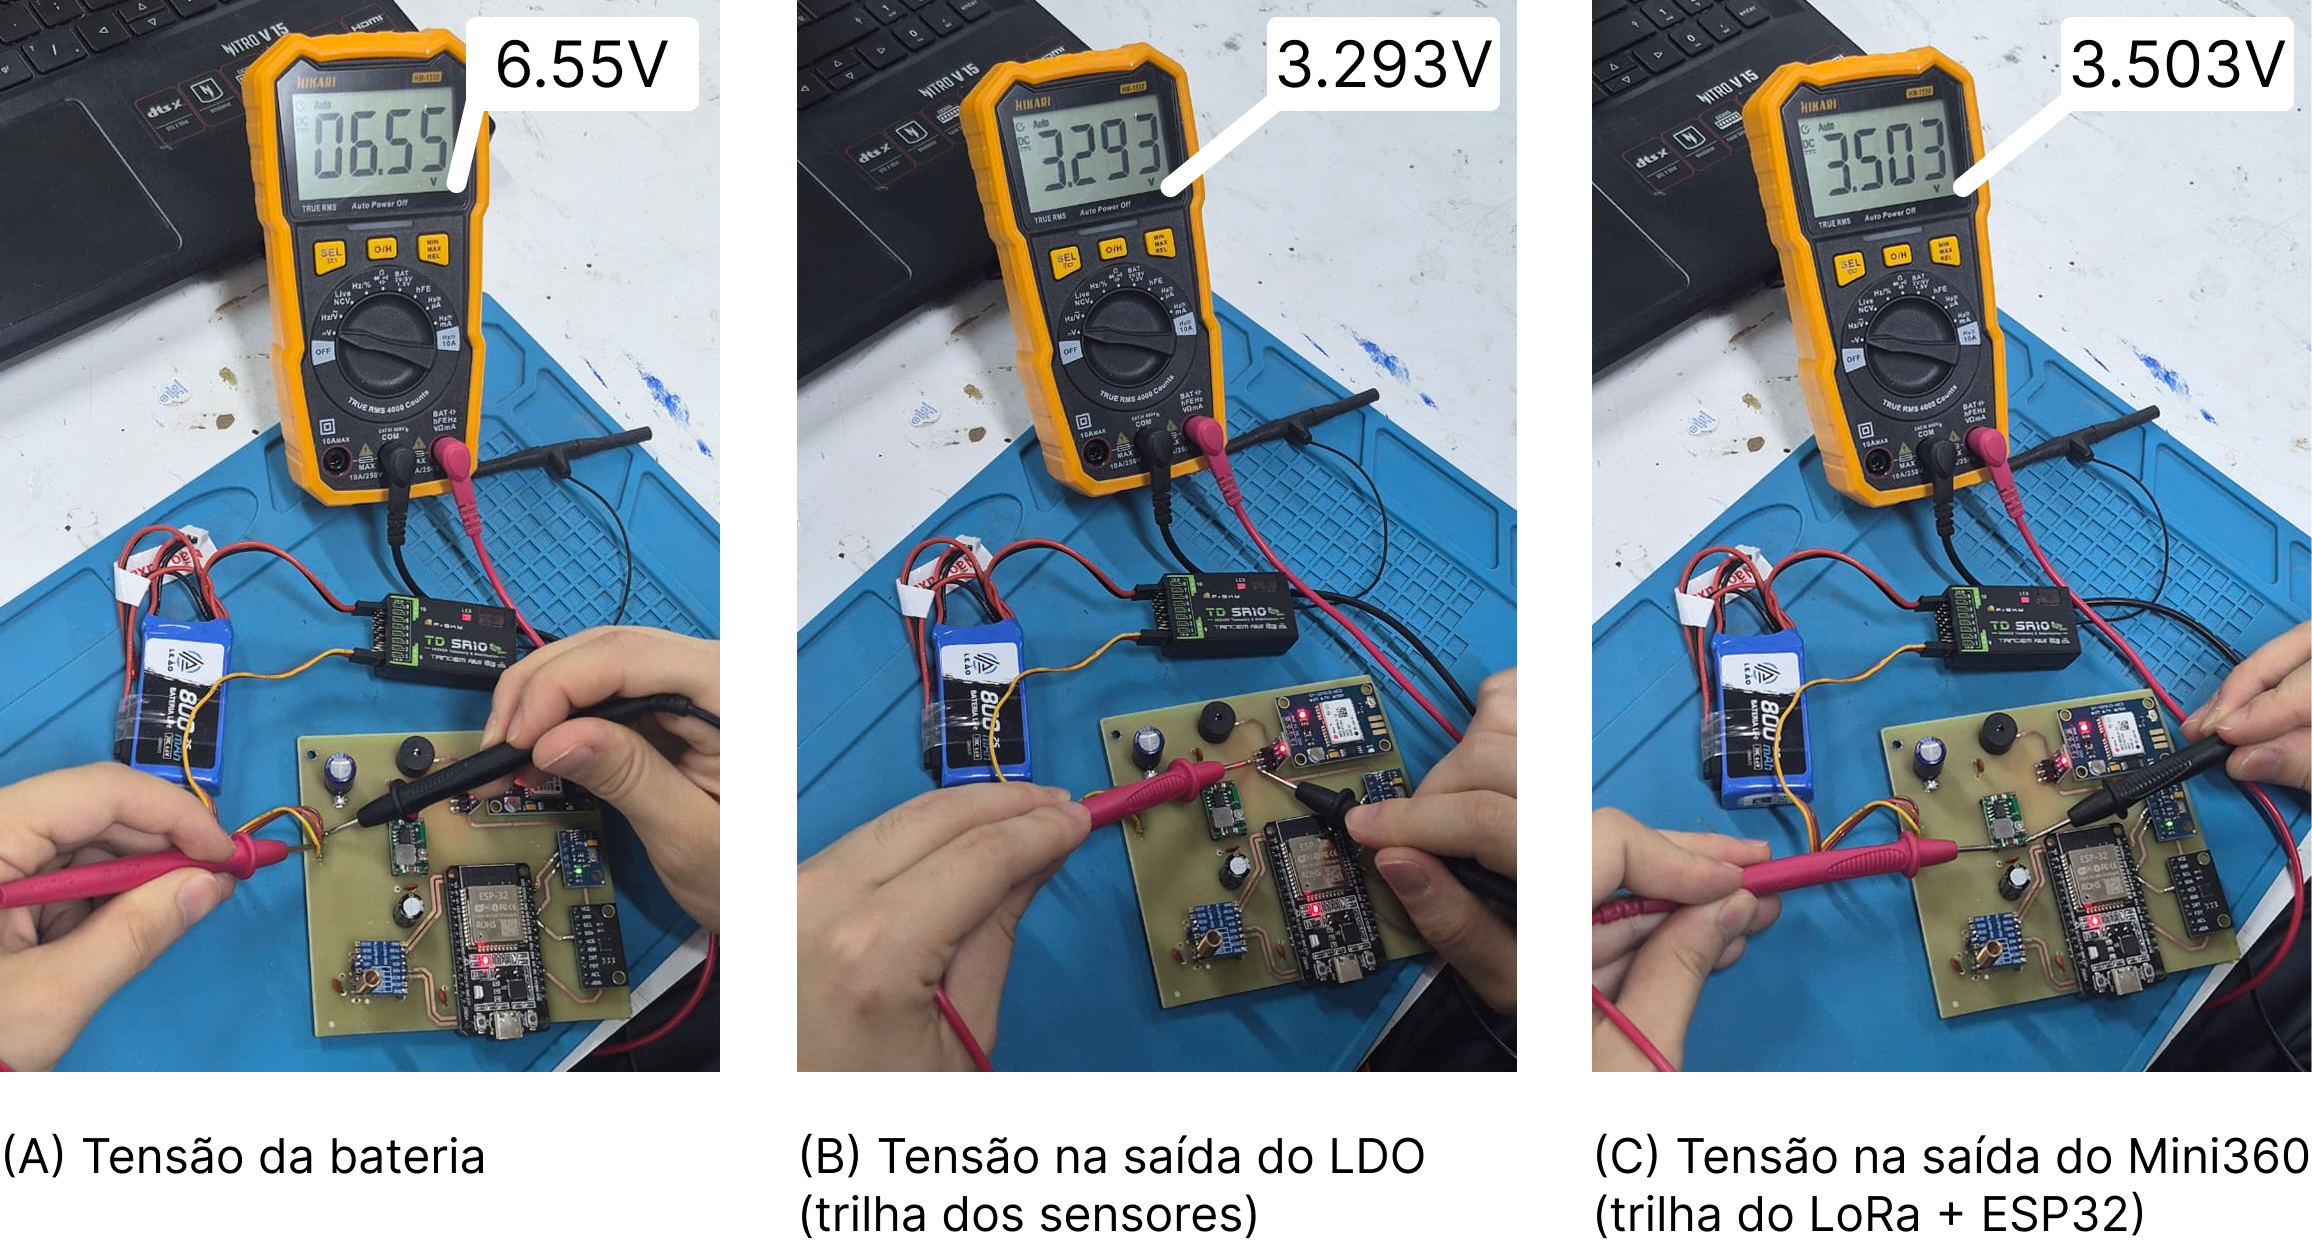
\includegraphics[width=1\textwidth]{images/tensao_pcb.png}\\
    \footnotesize Fonte: Autoria própria, 2026.
\end{figure}

No que tange ao perfil de consumo energético, o sistema foi monitorado em regime contínuo de captura sensorial e emissão de dados via radiofrequência. A instrumentação de medição indicou que o \textit{hardware} embarcado demanda uma corrente média de aproximadamente $0,033 A$ durante a maior parte do ciclo de execução. Contudo, a análise da curva de carga revelou a ocorrência de picos transitórios de corrente que atingem até $0,89 A$, conforme Figura \ref{fig:grafico_corrente}. Essa elevação abrupta e momentânea é uma característica esperada da modulação física do transceptor LoRa SX1276 (configurado para potência máxima de transmissão no estágio \textit{PA\_BOOST}), reafirmando a necessidade do barramento capacitivo e do conversor chaveado exclusivo para suprir as demandas instantâneas de rajada sem desestabilizar o barramento lógico primário.

\begin{figure}[ht]
    \centering
    \caption{Corrente do Sistema Embarcado ao Longo do Tempo}
    \label{fig:grafico_corrente}
    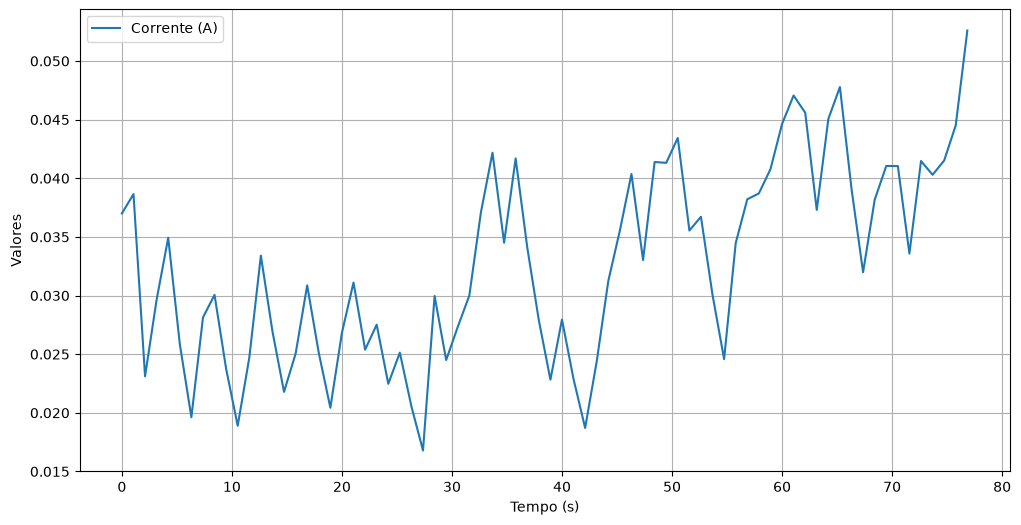
\includegraphics[width=1\textwidth]{images/corrente_embarcado.png}\\
    \footnotesize Fonte: Autoria própria, 2026.
\end{figure}

Por fim, a resiliência da arquitetura foi submetida a um ensaio de estresse com o sistema de telemetria integrado à malha de potência do sistema de controle da aeronave. O objetivo desta avaliação foi identificar potenciais afundamentos de tensão (\textit{sags}) ocasionados pelo acionamento concorrente dos servomotores e da comunicação. A análise do registro gráfico do teste indicou que, mesmo sob carga integrada, a tensão do barramento principal não decaiu consistentemente para valores inferiores a 5,0 V, conforme Figura \ref{fig:grafico_sistema_controle}.

\begin{figure}[ht]
    \centering
    \caption{Tensão e Corrente do Sistema de Controle}
    \label{fig:grafico_sistema_controle}
    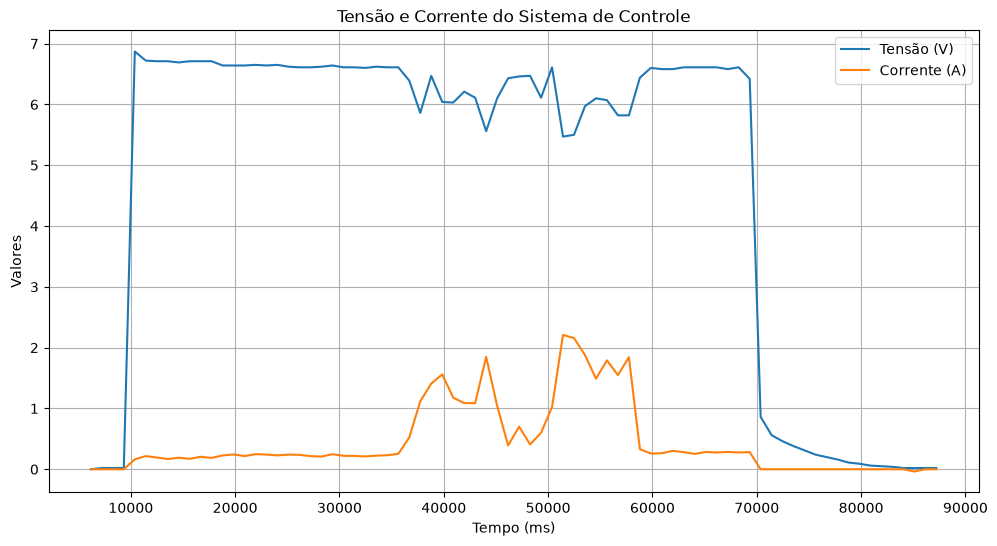
\includegraphics[width=1\textwidth]{images/grafico_sistema_controle.png}\\
    \footnotesize Fonte: Autoria própria, 2026.
\end{figure}

Ressalta-se, de forma crítica, que a taxa de amostragem inerente aos equipamentos de monitoramento utilizados para este ensaio específico pode mascarar quedas de tensão de alta frequência. Oscilações transientes na ordem de microssegundos podem não ter sido capturadas pelo histórico de medição. No entanto, a observação empírica corroborou a robustez do sistema elétrico: o microcontrolador operou sob constante monitoramento em modo \textit{debug} (via console) e não acusou, em momento algum, o acionamento do circuito supervisor de \textit{brownout detector} (BOD) ou reinicializações (\textit{resets}), comprovando que as flutuações de potência da aeronave não são suficientes para comprometer a estabilidade do \textit{firmware} de telemetria.


\section{Teste de Distância e Qualidade da Comunicação LoRa}

A confiabilidade do enlace de radiofrequência é um fator limitante para a operação segura de sistemas de telemetria aeroespacial. Para mensurar a resiliência da modulação LoRa adotada neste projeto, estruturou-se um ensaio de campo focado na avaliação da degradação do sinal — quantificada pelo Índice de Força do Sinal Recebido (RSSI) — em função do distanciamento geográfico entre a estação base e o nó transmissor.

O experimento foi conduzido em um ambiente comumente usado como pista de caminhada, onde a estação receptora, operando com o emulador HIL, foi fixada no ponto de origem. O operador portando o nó transmissor realizou um deslocamento linear progressivo até a marca de 500 metros de afastamento. O cenário de teste apresentou características de propagação não-ideais, englobando a presença de vegetação arbórea adjacente à pista e o trânsito esporádico de pedestres. Adicionalmente, as variações de relevo ao longo do trajeto culminaram na perda da linha de visada direta entre as antenas nos extremos da medição, emulando os piores cenários de atenuação esperados durante manobras de baixa altitude da aeronave.

A progressão da atenuação do enlace pode ser observada na Figura \ref{fig:grafico_rssi}, que correlaciona a queda dos níveis de RSSI com o aumento da distância \cite{haykin_communication}. Conforme previsto pela distância e agravado pelos obstáculos terrestres, o sinal apresentou um decaimento logarítmico. Contudo, o aspecto mais crítico da avaliação não reside apenas na potência bruta do sinal, mas na capacidade do receptor de decodificar a informação sob baixo limiar de sensibilidade.

\begin{figure}[ht]
    \centering
    \caption{Variação do RSSI ao Longo do Tempo e Distâncias Correspondentes}
    \label{fig:grafico_rssi}
    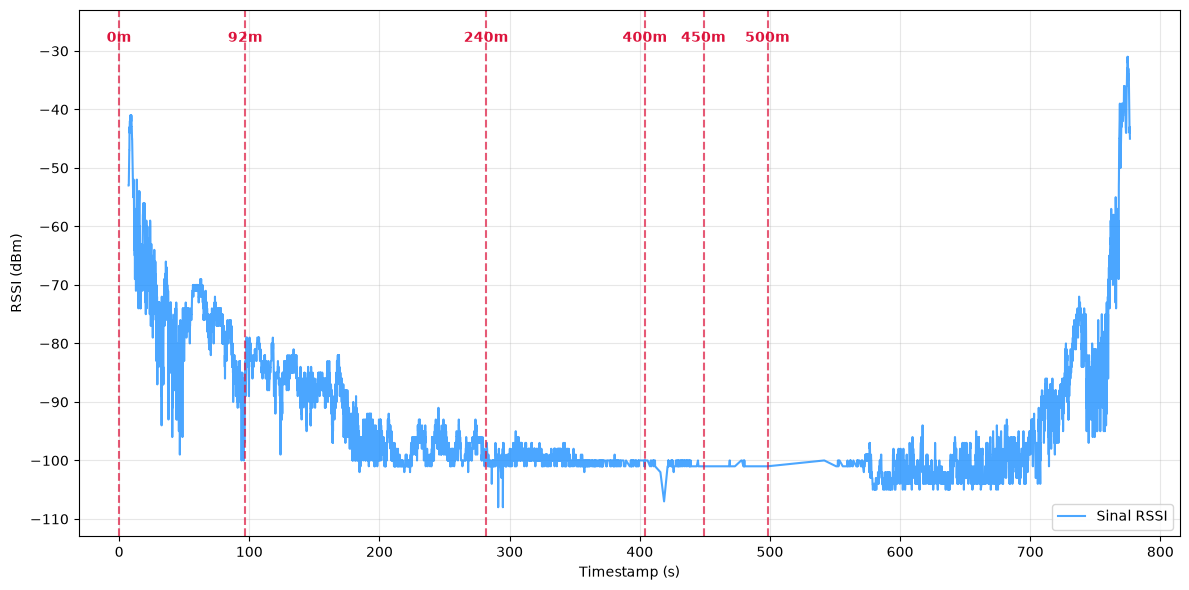
\includegraphics[width=1\textwidth]{images/grafico_rssi.png}\\
    \footnotesize Fonte: Autoria própria, 2026.
\end{figure}

A análise dos arquivos de \textit{log} da estação de solo revelou que, mesmo sob as condições adversas de bloqueio de visada e distanciamento de meio quilômetro, o índice de pacotes invalidados ou corrompidos limitou-se a apenas 1\% do volume total transmitido. Esta margem de erro restrita atesta a alta resiliência da modulação de Espalhamento Espectral por Chirp (CSS - \textit{Chirp Spread Spectrum}) inerente ao protocolo LoRa, que consegue recuperar a carga útil mesmo quando o sinal se encontra próximo ou abaixo do piso de ruído (\textit{noise floor}).

Os pacotes que efetivamente falharam na verificação de redundância cíclica (CRC) devido à corrupção de \textit{bits} foram adequadamente interceptados e descartados pelas rotinas de tratamento de exceção da camada \textit{middleware}, sem ocasionar travamentos no monitoramento geral. Conclui-se, portanto, que a arquitetura de comunicação satisfaz os requisitos do projeto, provendo um alcance operacional robusto que cobre com ampla margem de segurança os raios de giro e as distâncias típicas executadas em competições de aerodesign, onde o voo ocorre majoritariamente em campo aberto e com visada direta desobstruída.

	\chapter{Conclusões e Trabalhos Futuros}
\label{chap:conclusoes-e-trabalhos-futuros}

O desenvolvimento de veículos aéreos não tripulados, especialmente no contexto de competições de aerodesign, demanda o monitoramento rigoroso de variáveis cinemáticas e atmosféricas em tempo real para a validação de modelos aerodinâmicos e estruturais. Diante do alto custo e da natureza proprietária das soluções comerciais de instrumentação em voo, este trabalho propôs a concepção e implementação de um sistema de telemetria distribuído, estruturado de ponta a ponta, visando prover uma alternativa de baixo custo, alta modularidade e arquitetura aberta.

A síntese das etapas de desenvolvimento demonstra que o objetivo primário foi plenamente alcançado. A arquitetura foi fragmentada em três componentes funcionais integrados: o nó embarcado na aeronave, o middleware terrestre e a estação de controle em solo (Odin). No domínio embarcado, a integração de um microcontrolador de duplo núcleo (ESP32) com sensores inerciais (IMU), barométricos e de posicionamento global (GNSS) garantiu a aquisição quantizada dos dados sob estritas restrições elétricas e de peso. A transmissão dessas leituras operou sobre o protocolo LoRa operante em 915 MHz, estabelecendo um enlace de radiofrequência caracterizado por longo alcance e alta resiliência contra desvanecimentos.

Para o ambiente de solo, a introdução de um middleware dedicado atuou como um conversor eficiente de protocolos físicos, roteando o tráfego do espectro LoRa para uma rede local sem fio em formato de datagramas UDP. Esta decisão arquitetural isolou a estação de operação computacional das complexidades de baixo nível do rádio. Por fim, o software cliente cumpriu os requisitos de monitoramento ao adotar o padrão arquitetural Model-View-Controller (MVC), provendo uma interface orientada a eventos capaz de deserializar, renderizar gráficos de alta frequência e registrar os logs de voo de forma assimétrica, sem incorrer em bloqueios de processamento (thread-blocking).

A consolidação destes componentes, atestada pelos ensaios elétricos e pelas rotinas de simulação Hardware-in-the-Loop (HIL), confirmou a viabilidade técnica do sistema. Com uma taxa de fragmentação de pacotes contida em níveis operacionais aceitáveis (próxima a 1\%) e estabilidade funcional mantida sob condições de estresse na malha de potência, conclui-se que a solução entrega uma plataforma telemétrica robusta, pronta para amparar ensaios de voo práticos com a precisão e a confiabilidade exigidas pelo escopo do projeto.

\section{Contribuições Técnicas e Metodológicas}

Sob a ótica da engenharia de \textit{software} embarcado, a principal contribuição metodológica deste trabalho reside na aplicação da Arquitetura Hexagonal  na concepção do \textit{firmware} da aeronave. Em contraste com abordagens monolíticas comuns em projetos de instrumentação estudantil, a estruturação baseada na injeção de dependências promoveu um alto nível de desacoplamento, isolando rigorosamente a lógica de domínio — responsável pela quantização, escalonamento matemático e construção das máquinas de estados — das amarras físicas de \textit{hardware}. Como resultado direto, essa abstração viabilizou a execução de metodologias de teste em ambiente controlado, como o \textit{Hardware-in-the-Loop}. Esta capacidade de substituir as interfaces sensoriais por adaptadores emulados permitiu a injeção de perfis de voo sintéticos, garantindo a validação exaustiva do sistema e a mitigação de falhas de \textit{software} de forma antecipada e segura.

Do ponto de vista da arquitetura de sistemas e de redes de comunicação, o projeto demonstra mérito ao inserir uma camada de \textit{middleware} terrestre operando como ponte translatora entre a radiofrequência sub-GHz e a rede local de alta capacidade. A delegação da recepção física dos pacotes LoRa e do subsequente encapsulamento em datagramas UDP a um nó microcontrolado isentou o computador da estação de controle (Odin) da severa sobrecarga de processamento associada à escuta contínua de barramentos seriais (UART/USB) em baixo nível.

Esta segmentação arquitetural proporcionou um fluxo de dados limpo e padronizado via \textit{sockets} de rede, permitindo que a aplicação cliente operasse de forma totalmente assíncrona. Consequentemente, o uso desta topologia descentralizada revelou-se uma solução eficaz para evitar gargalos comuns em sistemas de recepção direta, assegurando que o processamento do computador de solo estivesse integralmente dedicado à renderização gráfica a 20 Hz e à gravação redundante dos pacotes MAVLink em disco, sem comprometer a latência ou o acúmulo de dados.


\section{Limitações Encontradas}

A despeito dos resultados satisfatórios alcançados e da validação funcional da arquitetura, o desenvolvimento e a experimentação deste projeto esbarraram em limitações inerentes às restrições de escopo, de instrumentação laboratorial e das próprias tecnologias adotadas. O reconhecimento destas restrições é fundamental para a avaliação crítica do sistema e para o balizamento das expectativas em cenários de operação reais.

A primeira limitação evidente manifestou-se na camada física de comunicação. Embora a taxa de invalidação de pacotes de 1\% ateste a resiliência do protocolo LoRa sob condições adversas, ela confirma a suscetibilidade do enlace sub-GHz a obstruções na primeira Zona de Fresnel e à perda da linha de visada direta (LoS). Em cenários de voo que envolvam a interposição de relevo acidentado denso ou estruturas urbanas entre a aeronave e a base, a degradação do sinal pode escalar, indicando que a solução atual, baseada em antenas omnidirecionais simples, possui um limiar de saturação em ambientes de forte obstrução.

No escopo da validação elétrica do sistema embarcado, identificou-se uma limitação técnica significativa relacionada aos equipamentos de medição empregados. Consequentemente, o aparato experimental foi incapaz de capturar quedas de tensão transientes de altíssima frequência que podem ser induzidas pelo acionamento abrupto dos servomotores da aeronave. Embora o circuito supervisor interno do microcontrolador não tenha registrado reinicializações, a ausência de análises com osciloscópios de alta velocidade impede a garantia de imunidade a transientes eletromagnéticos severos.

Por fim, no que tange à infraestrutura física, a montagem estrutural do componente \textit{middleware} apresenta restrições mecânicas. A decisão de instanciar o circuito de recepção terrestre sobre \textit{protoboards} com condutores rígidos foi justificada pela imobilidade da estação e pela facilidade de manutenção em bancada. Contudo, essa topologia carece da robustez mecânica e da blindagem contra interferências eletromagnéticas (EMI) inerentes a uma Placa de Circuito Impresso (PCB) dedicada. Em um ambiente de pista de voo, a exposição a vibrações acidentais ou manuseio contínuo eleva o risco de mau contato nos terminais, o que poderia comprometer temporariamente o roteamento dos pacotes para a rede local da estação de controle.


\section{Trabalhos Futuros}

Como consequência natural do ciclo de desenvolvimento e visando o amadurecimento contínuo da arquitetura proposta, elenca-se um conjunto de diretrizes para a evolução do sistema. 

No escopo do \textit{hardware}, recomenda-se a transição dos protótipos experimentais para Placas de Circuito Impresso dedicadas a nível de \textit{Surface Mount Device} (SMD), abrangendo tanto o nó embarcado na aeronave quanto o componente de \textit{middleware} terrestre. Esta evolução construtiva é necessária para garantir a miniaturização física, a redução da massa estrutural e, criticamente, a mitigação de interferências eletromagnéticas em malhas de alta frequência. Ademais, a base sensorial da aeronave pode ser expandida através da integração de instrumentos específicos de dinâmica de fluidos, como um tubo de Pitot acoplado a um transdutor de pressão diferencial, viabilizando a medição direta da velocidade aerodinâmica relativa.

No que tange ao \textit{software}, sugere-se uma exploração mais aprofundada das capacidades operacionais da camada de \textit{middleware}. O microcontrolador de solo pode ter sua responsabilidade expandida para atuar além de um roteador passivo de protocolos. A implementação de lógicas de processamento de borda (\textit{edge computing}) no \textit{middleware} permitiria a pré-filtragem de pacotes corrompidos, a análise da qualidade de serviço (QoS) do enlace LoRa em tempo real e a agregação de estatísticas de conexão antes da retransmissão dos datagramas via UDP, otimizando o consumo de banda na rede local da estação.

Para o aprimoramento dos métodos de verificação, propõe-se a adoção de processos formais de qualidade de \textit{software} e de metodologias consolidadas de engenharia. A implementação de rotinas de testes unitários focadas estritamente na camada de domínio garantirá a corretude matemática contínua das rotinas de quantização e conversão de escalas. Em paralelo, a adoção da Engenharia de Sistemas Baseada em Modelos (MBSE) proverá uma estrutura analítica rigorosa para a rastreabilidade de requisitos, gestão de interfaces e controle do ciclo de vida do projeto, mitigando o risco de regressões arquiteturais em iterações futuras do código.

Por fim, a infraestrutura de comunicação concebida pode ser expandida para unificar todo o ecossistema de dados em voo da equipe. A arquitetura modular desenvolvida permite que outras frentes de instrumentação, como estações portáteis de aquisição de dados climáticos para aferição de densidade do ar na pista, sejam integradas de forma transparente à plataforma unificada. Ao padronizar a saída desses novos nós sensores para o protocolo MAVLink e roteá-los através da malha UDP existente, a estação de solo será capaz de correlacionar variáveis ambientais exógenas com o desempenho cinemático da aeronave, enriquecendo profundamente a capacidade de análise pós-voo sem demandar reestruturações profundas no \textit{software} base.

	
	%Elementos pós-textuais	
 \bibliographystyle{abntex2-alf}
	\bibliography{3-pos-textuais/referencias}
%	\imprimirglossario	
	 \imprimirapendices
		% Adicione aqui os apendices do seu trabalho
		\input{3-pos-textuais/apendices/apendice-a}
	 \imprimiranexos
		% Adicione aqui os anexos do seu trabalho
		\anexo{Exemplo de um anexo}
\label{an:ex_anexo_a}

Anexo é um texto ou qualquer tipo de documento utilizado para complementar um trabalho acadêmico em sua argumentação, porém, sendo este documento de autoria de terceiros.
	\imprimirindice

\end{document}
